\chapter{Background}

This chapter starts with a brief comparison between grids and cloud computing. Next, it gives an overview of the current state of the workflow engine ecosystem by looking at some of the existing platforms with a focus on the execution environments they support, and cloud deployments in particular. This leads to the last section, where we investigate tools and frameworks that could allow deploying a cluster in the cloud and scheduling jobs on the respective instances.

\section{Grids and Cloud Computing}

Ever since the early days of high performance computing, researchers have been running resource-intensive experiments and simulations on supercomputers, machines with hundreds of thousands of cores and high parallelisation capabilities \cite{Supercomp}. However, in the last two decades the extensive costs and restricted access to such systems have shifted computation towards local clusters and grids.

Grids are distributed networks of remote computers crowdsourced in general from academic communities. They harness unused resources in the infrastructure and are managed through middleware software (e.g. EMI\footnote{European Middleware Initiative} \cite{EMI}) that coordinates incoming computation across the machines they interconnect \cite{Myerson}. Access to grids is usually free and restricted to research projects.

Although clouds evolve from grids and both aim to achieve similar goals in the area of distributed computing, there are some substantial differences in terms of features and how they operate \cite{Juve2009, Myerson, CloudsGrids}:

\begin{itemize}
	\item Clouds offer on-demand provisioning of resources. This enables users to easily scale infrastructures hosted in the cloud by simply requesting more instances as resource requirements grow. They create an illusion that resources can be provisioned infinitely by functioning at such a large scale that they can fulfil practically any demands.
	\item As opposed to grid operators, cloud providers are generally commercial and charge users on a pay as you go basis. Usage is usually measured in hours per instance and the business model creates no upfront planning or costs for users. Since they are paid services, cloud providers also offer better reliability and uptime guarantees. Private clouds can also be set up for users that want to abstract away their pool of resources but are concerned about security of their data.
	\item Clouds are particularly suitable for hosting long-running jobs, such as web servers. In this case, users can easily take advantage of features such as automatic scaling, where more servers are automatically provisioned to match abrupt increases or decreases in the number of incoming requests.
	\item Virtualisation is used extensively in clouds and it permits running legacy software that has very strict environment requirements. Although they might be sharing a physical machine with other consumers, users can fully customise the virtual runtime in isolation by choosing the operating system and libraries they need. Consolidating a homogeneous fleet of machines is also straightforward, since snapshots of a runtime environment can easily be ported to other instances.
\end{itemize}

Considering the advantages listed above and growing support for cloud services, they are a good fit for the deployment of workflow management systems. However, as discussed in the next section, current workflow platforms do not take full advantage of advanced cloud features such as automatic scaling.

\subsection{Amazon Web Services}

Since the project primarily aims at supporting Amazon EC2 as a target environment for running experiments via OpenMOLE, this subsection briefly describes some of the basic terminology related to Amazon's cloud services:

\begin{itemize}
	\item \textit{AWS}\footnote{Amazon Web Services} \cite{AWS} is the whole suite of services provided by Amazon as part of its cloud platform.
	\item \textit{EC2}\footnote{Elastic Compute Cloud} \cite{EC2} is the cloud service that provides on-demand computational resources.
	\item \textit{EC2 Spot Instances} are normal EC2 instances that are temporarily free and are auctioned by Amazon. The highest bidder retains the right to use the resources.
	\item \textit{S3}\footnote{Simple Storage Service} \cite{S3} is a general-purpose persistent file storage service.
	\item \textit{EBS}\footnote{Elastic Block Store} \cite{EBS} concerns storage volumes that are attached to machines provisioned through EC2.
	\item An \textit{AMI}\footnote{Amazon Machine Image} is a snapshot of the environment on an EC2 machine. New EC2 instances can easily be created from a given AMI.
\end{itemize}

\section{Workflow Platform Ecosystem}

Chronologically, scientific workflow systems have emerged from the bioinformatics community along with the recent trend towards data-driven research. Their large number and segregation despite achieving similar purposes could be explained by many research groups independently trying to formalise, consolidate and generalise their workflows. Therefore, most systems achieve comparable goals, with slight variations. Common features include \cite{Goble2009}:

\begin{itemize}
	\item Creation and definition of reusable tasks or work units. A task can represent anything from processing an image to running an expensive computation or invoking a service over the web.
	\item A graphical user interface that simplifies the flow of tasks by allowing definitions via a simple visual representation. See Figure \ref{OpenMOLEGUI} for an example of this.
	\item An execution platform that runs the workflow, hiding the complexity of calling service applications, managing and storing data, setting up and consuming remote computational resources, dealing with failures and logging results and unexpected behaviours. This is the engine of the application.
	\item A collaboration platform, where users can interact and share workflows.
\end{itemize}

\begin{figure}[h]
	\centering
		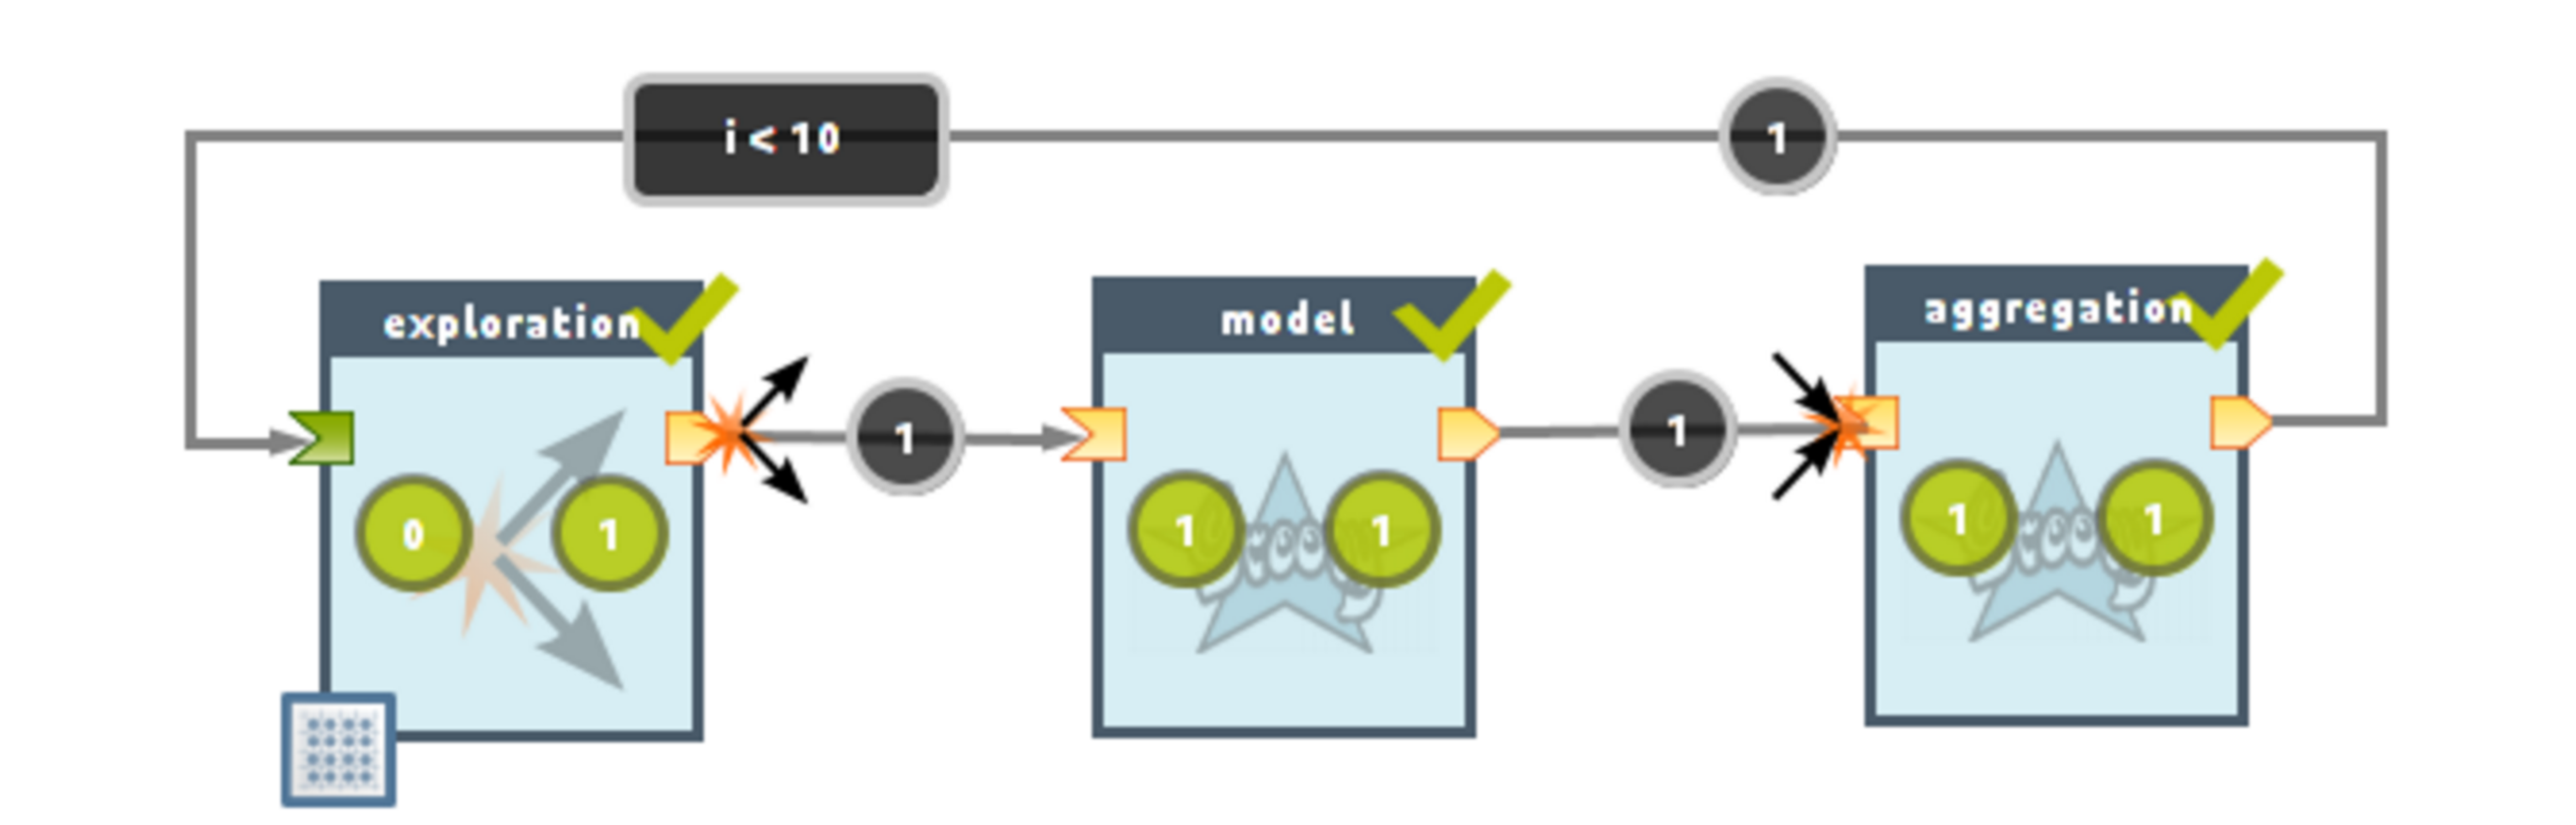
\includegraphics[scale=0.30]{OpenMOLEGUI.png}
	\caption{OpenMOLE graphical workflow \cite{Reuillon2012}.}
	\label{OpenMOLEGUI}
\end{figure}

From the multitude of existing workflow systems, we have selected some of the most often referenced ones for closer inspection. Since our focus only spans the targeting of different remote execution platforms, we will generally omit the details of workflow definition and the underlying implementation, as well as the graphical design and collaboration factors. We are particularly interested in engines that support cloud environments and insights we can draw from their design and infrastructure.

\subsection{Taverna}

Taverna \cite{Wolstencroft2013} is one of the most popular workflow systems. It was initially created as a framework for bioinformatics research and has remained used primarily in this field despite efforts from contributors towards expansion to other research areas.

The system has three main functional components:
\begin{itemize}
	\item \textit{Taverna Workbench} is the standard suite including the user interface and execution platform. However, this package alone is quite restricted since it only supports running the workflow locally and not distributing it remotely.
	\item \textit{Taverna Server} is a suite that works on the principles of simple client-server interaction. A server instance stores workflow blueprints created by the community and the client is only allowed to trigger runs of the experiments via a web interface. In this model, only server administrators have permission to add workflow content, while regular users are not allowed to freely create and upload their own custom workflows to the server. Additionally, the need for a full installation and configuration of the server software in order to execute work remotely limits ease of deployment and creates an important entry barrier.
	\item \textit{Taverna Player} is the web interface used by the client to send requests to Taverna Server.
\end{itemize}

Despite its maturity, Taverna does not, on its own, have built-in support for automatic server installations on grids or clouds. Instead, users need to develop custom orchestration infrastructure for these environments to allow deploying clusters coordinated by the instance where Taverna Server is installed. Both caGrid \cite{caGrid} and BioVeL \cite{BioVeL} have implemented such solutions \cite{TavernaGrid, Donvito} to take advantage of grid resources. On Amazon EC2, Taverna is only available as an Amazon Machine Image (AMI) runnable on a single instance, without support for distributed execution.

\subsection{Galaxy}

Galaxy \cite{Goecks2010} is another community specific web-based platforms for managing workflows, focussing on genomic research. Conceptually, it is driven by the motivation to ensure accessibility of computational resources by providing researchers with simple web interfaces to interact with distributed environments, reproducibility of experiments by tagging and recording order and intent of each action users take, as well as transparency of findings by consolidating a robust collaboration framework.

CloudMan \cite{Afgan2010} is the cloud resource management tool used by Galaxy to instantiate pre-packaged clusters on Amazon EC2 machines. To achieve this, the user needs to use the AWS Management Console to request from an instance that will be used as the master node of a new SGE cluster. Next, the number of slave instances in the cluster can be adjusted using the CloudMan Console, as shown in Figure \ref{CloudManConsole}.

\begin{figure}[h]
	\centering
		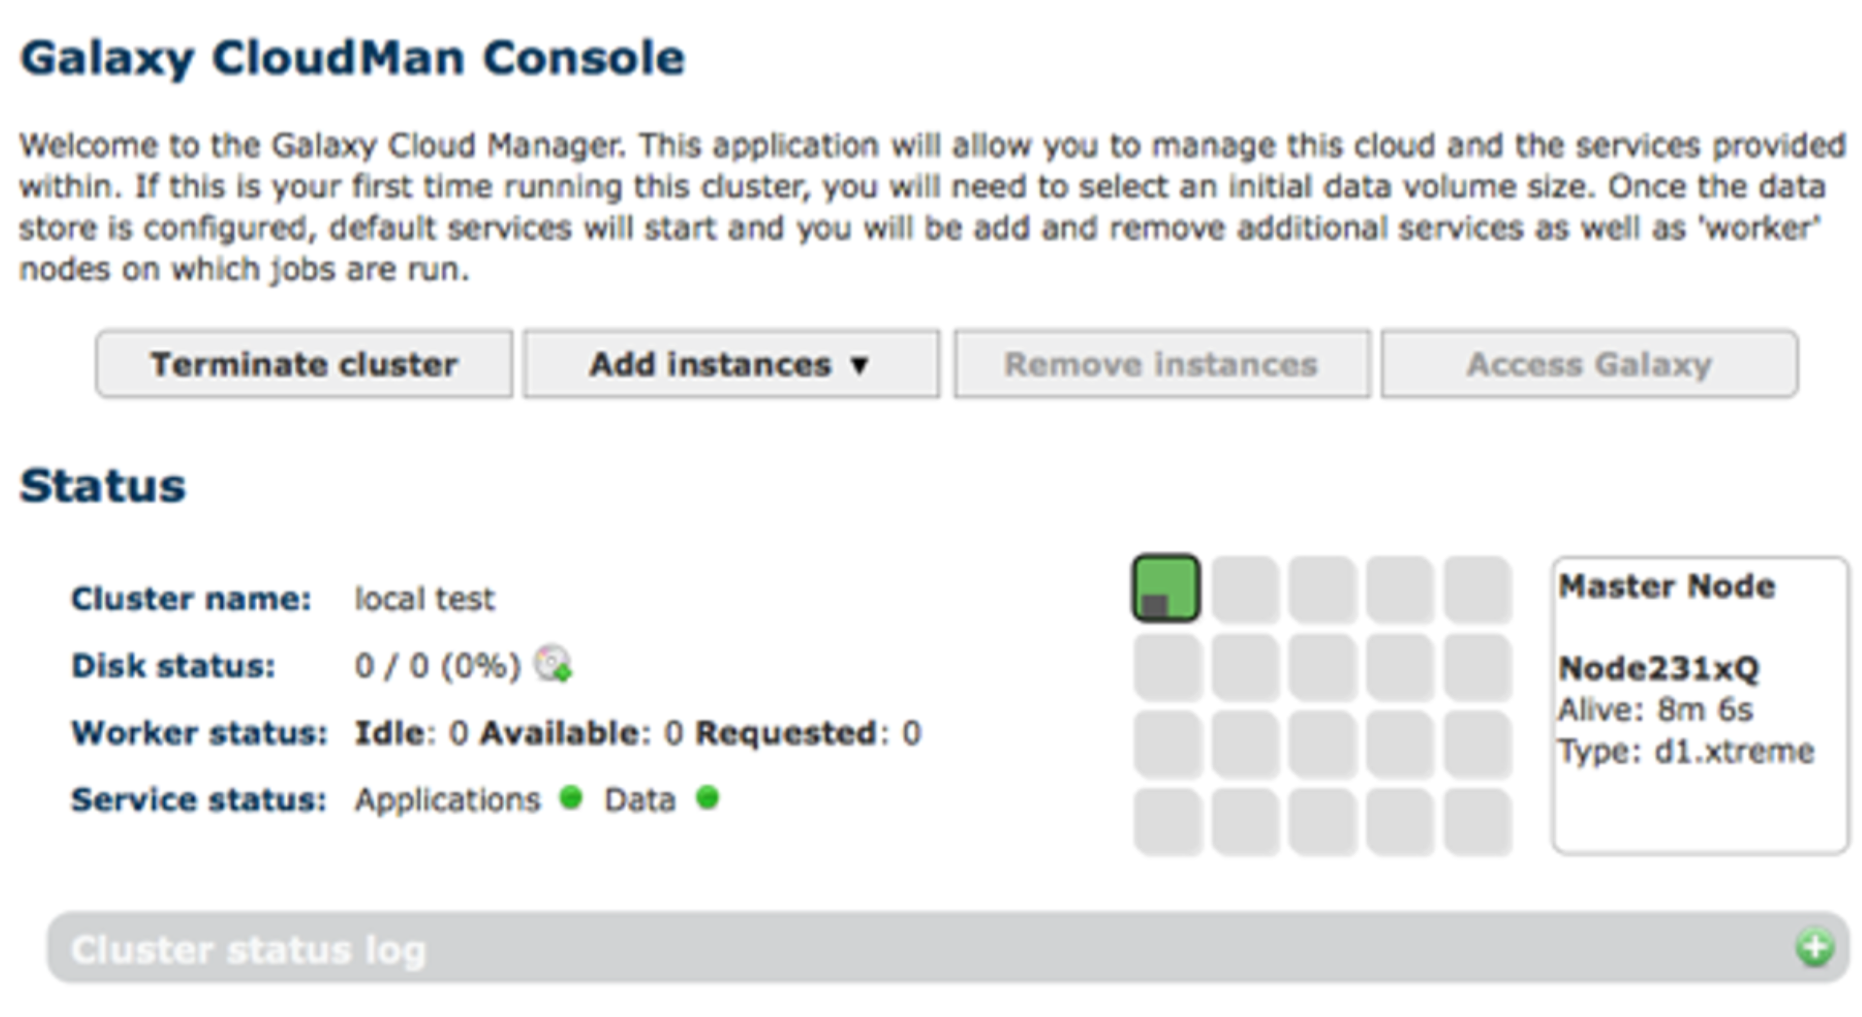
\includegraphics[scale=0.37]{CloudManConsole.png}
	\caption{CloudMan cluster management console \cite{Afgan2010}.}
	\label{CloudManConsole}
\end{figure}

Since EC2 instances do not save data on disk by default, persistence on Amazon Elastic Block Storage can be explicitly turned on from the CloudMan Console. CloudMan also deals with cases when the initial capacity of an EBS volume attached to the master instance is exceeded by safely pausing activity in the cluster before reattaching a new expanded capacity volume and resuming work. However, the job submission system still does not achieve full automation, since it requires a human to manually turn on the master node in the cluster, as opposed to the system being brought up on the fly and turned off on workflow termination. This is a problem in the context of EC2 or other commercial clouds, since it means that the user might continue to be charged for resources that are no longer being used.

One major advantage of CloudMan is its modular architecture, under which instances only use a lightweight AMI and reference the tools they need from external storage such as EBS, as shown in Figure \ref{CloudManArch}. This grants further flexibility in terms of updating the system, because the AMI does not need to be repackaged frequently and the state of machines can be modified by simply writing on persistent storage.

\begin{figure}[h]
	\centering
		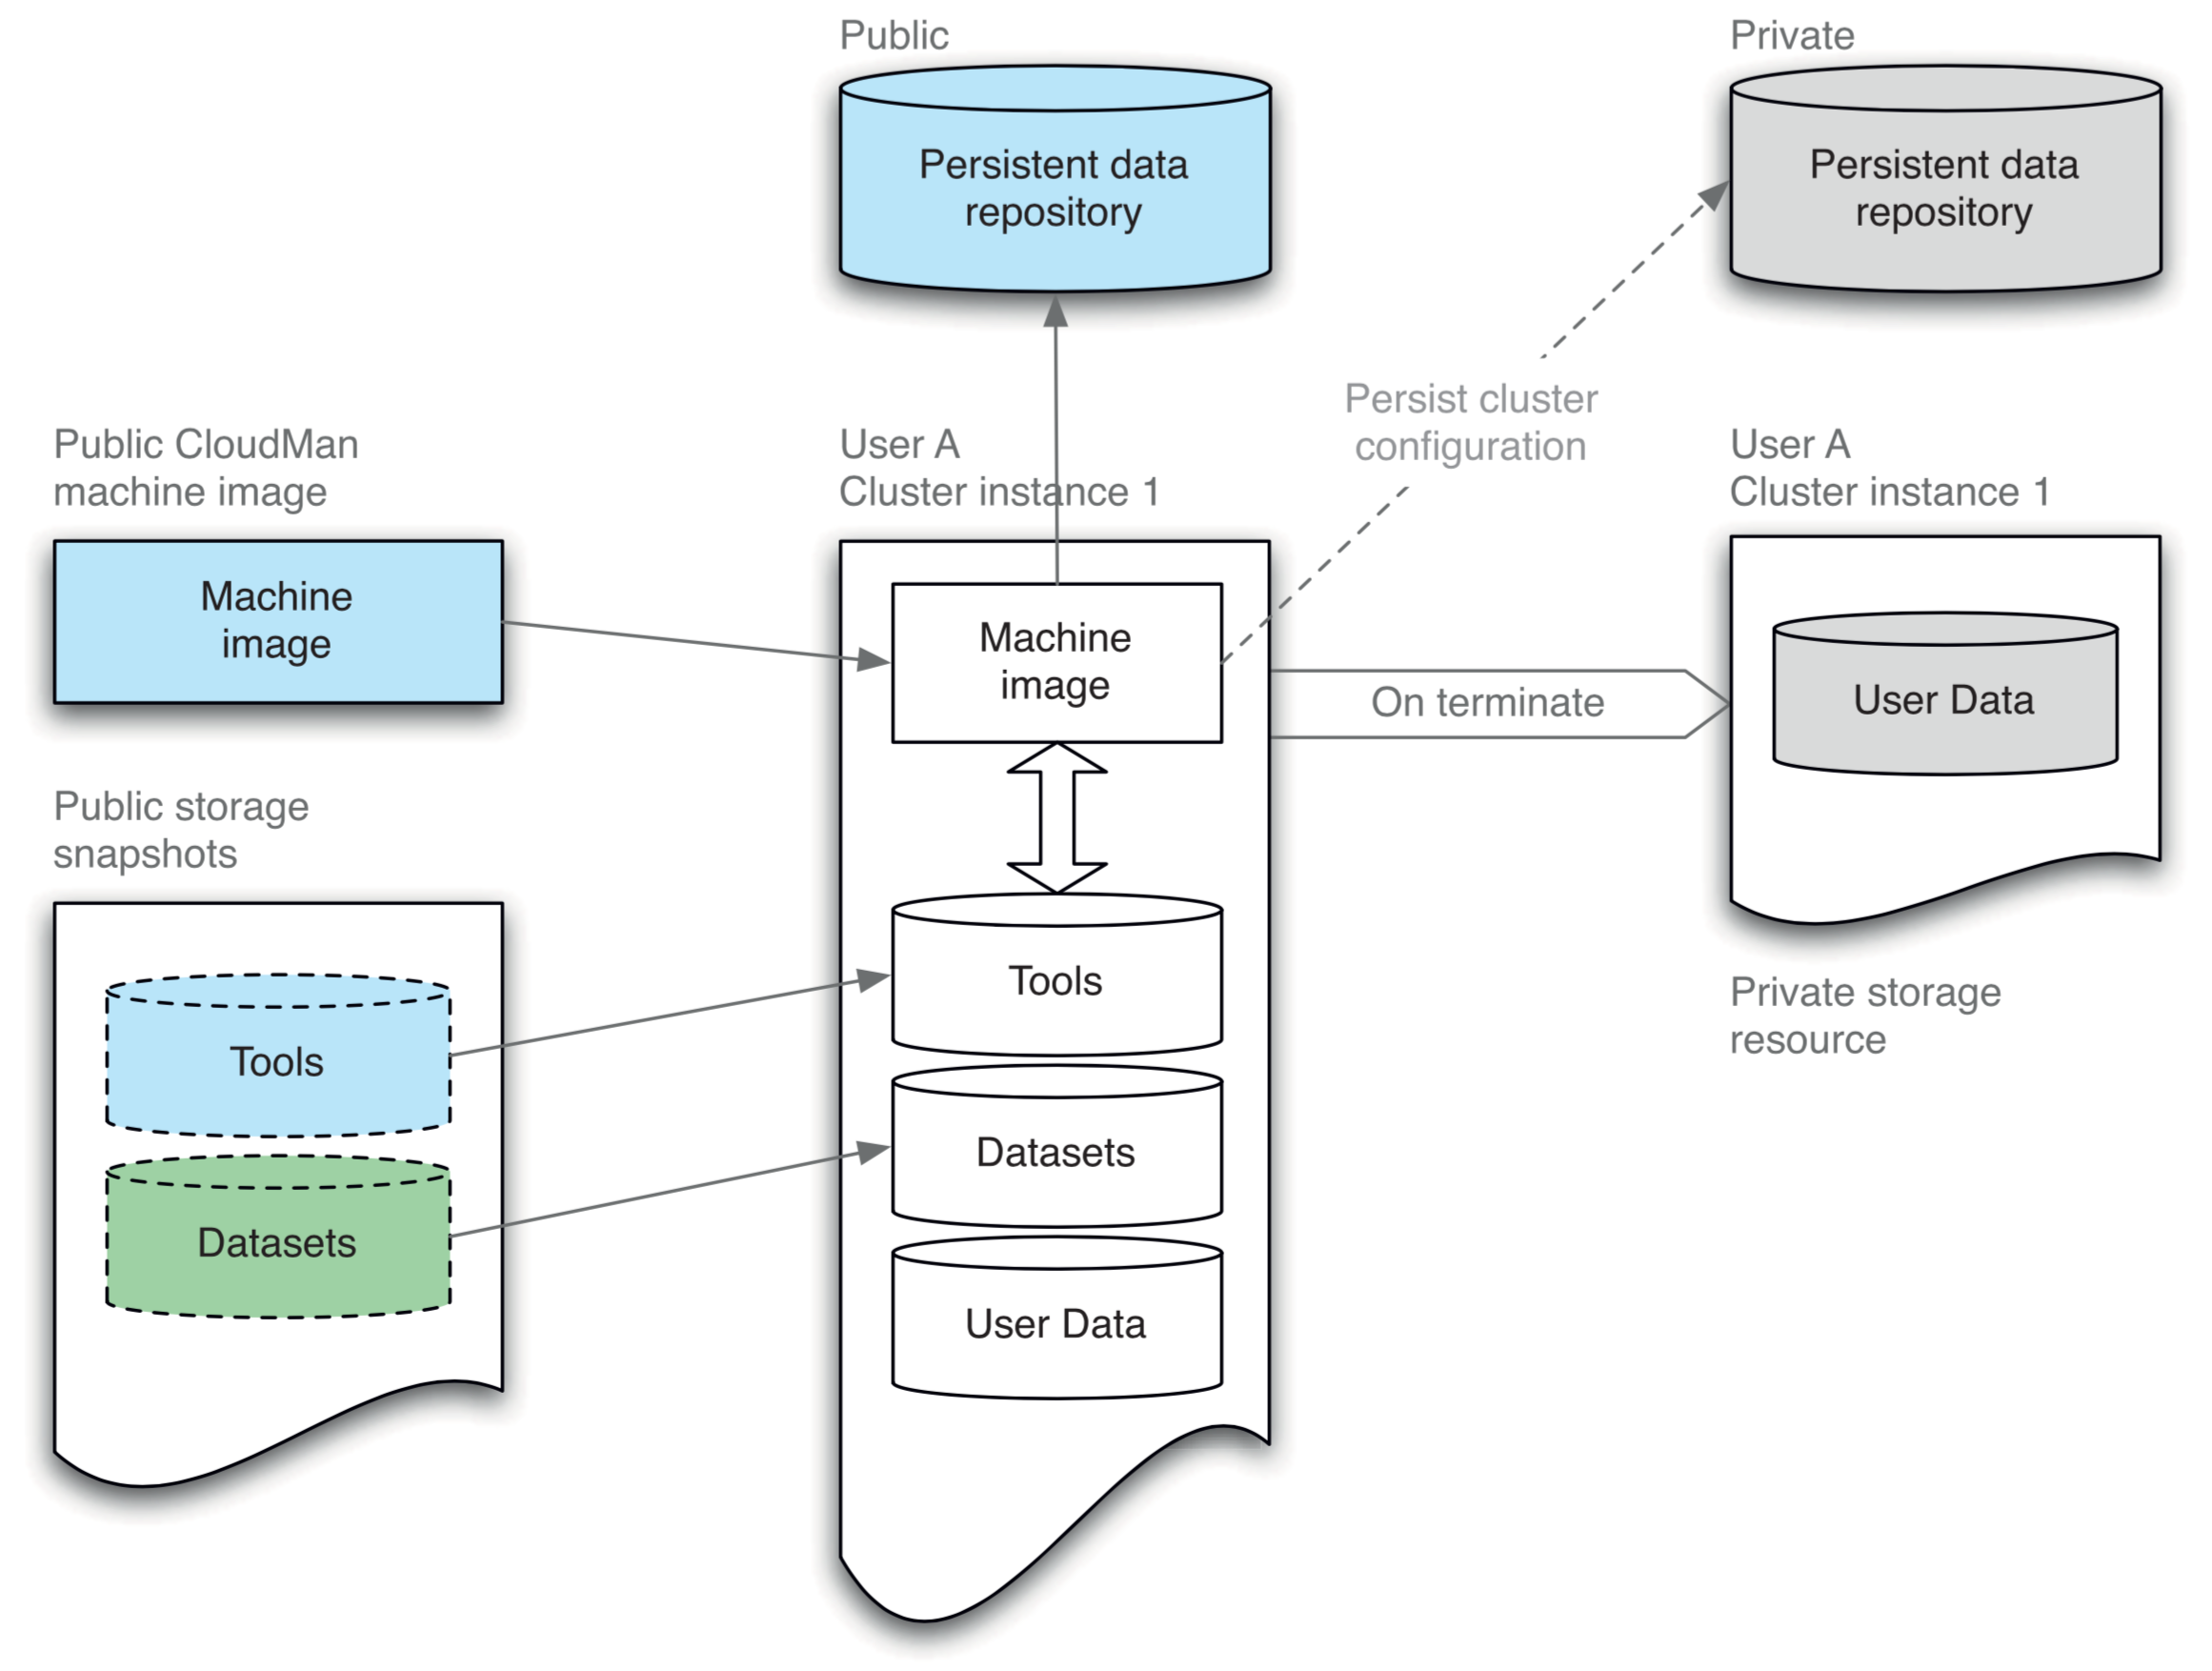
\includegraphics[scale=0.35]{CloudManArch.png}
	\caption{CloudMan modular architecture \cite{Afgan2010}.}
	\label{CloudManArch}
\end{figure}

\subsection{Tavaxy}

Tavaxy \cite{Abouelhoda2012} was created from the desire to ease the sharing of scientific workflows between the increasingly large user bases of Taverna and Galaxy within the bioinformatics community. The limited interoperability between the two systems was caused by differences in workflow description languages, as well as execution engines and overall design. Tavaxy consolidates Taverna and Galaxy workflows to run and be edited in a single environment, encouraging the community to create composite routines with building blocks from both worlds.

Tavaxy focuses on efficiently and transparently delegating workload to grid and cloud platforms. It can run a cluster when it is provided with a distributed file system similar to NFS and a standard job scheduler like SGE. The preferred cloud platform is Amazon EC2 and provisioning extra resources is done via a simple web interface, operated similarly as for Taverna and Galaxy.

\begin{figure}[h]
	\centering
		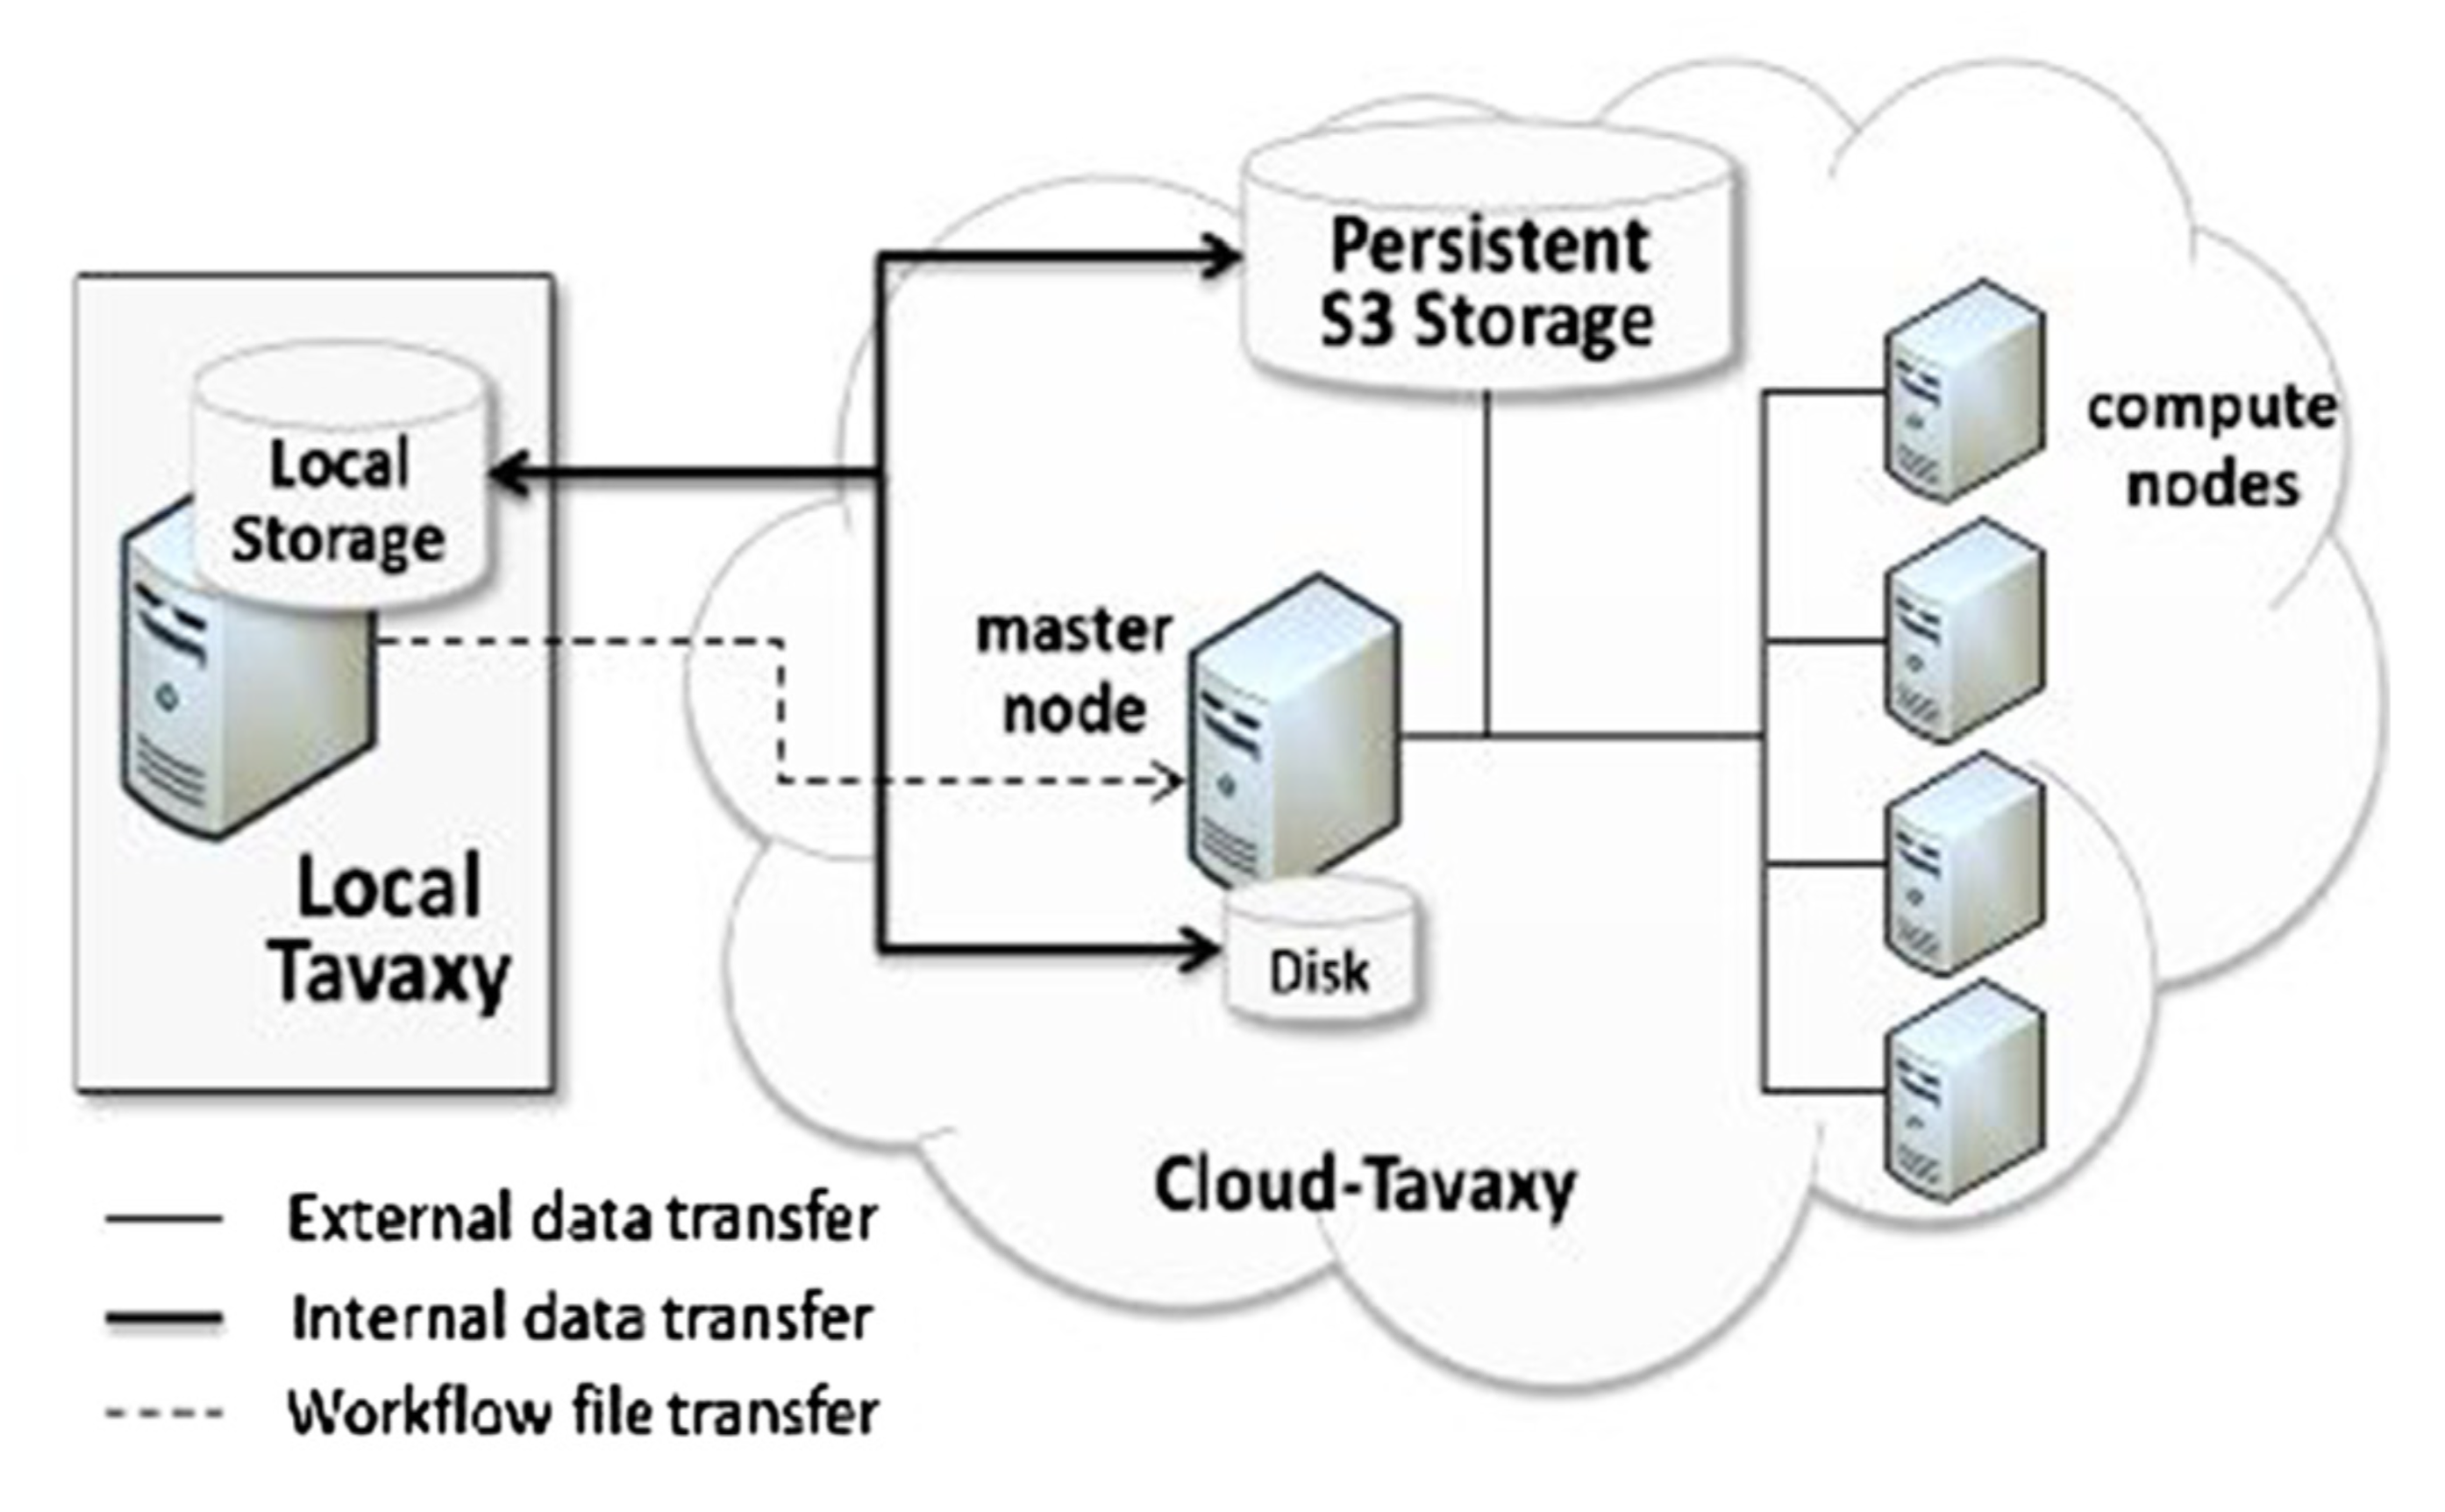
\includegraphics[scale=0.25]{TavaxyArch.png}
	\caption{Tavaxy interaction between a local machine and Amazon EC2 \cite{Abouelhoda2012}.}
	\label{TavaxyArch}
\end{figure}

Three different modes are available for delegating computation to EC2:

\begin{itemize}
	\item \textit{Whole system instantiation}, where the user has no local version of Tavaxy installed and can bootstrap a new instance from a provided AMI. This will automatically create and configure a cluster that the user can control through a web console. Amazon S3 \cite{S3} is used for persistent storage of shared data in the cluster.
	\item \textit{Sub-workflow execution}, which presumes a local installation and Tavaxy used for workflow design and allows the user to create a cluster in the cloud from a more lightweight AMI wrapping the runtime environment. The local machine sends the workflows remotely for execution and waits for results of the run. The user has two options for transmitting the input data and persisting the results. The first option is to send Inputs along with the workflow definition to master node machine and save outputs manually to local storage. The alternative is to upload input data to S3 and configure the cluster to direct reads and writes to S3 directly. The general architecture for this mode of operation can be observed in Figure \ref{TavaxyArch}.
	\item \textit{Single task instantiation}, which is similar to sub-workflow execution, except that only a task in the workflow is delegated to the cloud.
\end{itemize}

\subsection{Kepler}

Kepler \cite{Kepler} is one of the first general-purpose scientific workflow systems, recognising the need for transparent and simplified access to high performance computing platforms more than a decade ago. It also underlined concepts such as reusable and reproducible workflow runs, scalability of models, as well as fault tolerance and reliability in the context of remote execution \cite{Ludascher2006}.

The novelty of Kepler's design resides in the actor-oriented model. Actors are basic independent components representing either data sources or operations in the workflow. They are interconnected via channels and own receivers that handle their external communication, as well as input and output ports.

However, the execution model differs from standard systems in that its flow is not directed by the topology of the network. Instead, a special component named \textit{director} establishes the order of execution for actors, selects the operations they perform and orchestrates their communication by controlling their respective receivers \cite{Curcin2008}. This means that actors are not necessarily executed sequentially but are triggered by data received on incoming ports. Such as design reveals possibilities for concurrency semantics and renders the model fit for embedded systems simulations.

Although Kepler does not support execution on clusters in cloud environments out of the box, research groups using it have developed custom solutions to partially support this functionality. Wang and Altintas \cite{Wang2012} propose EC2 actors capable of managing Amazon virtual machines and suggest using StarCluster \cite{StarCluster} to build virtual clusters from the Kepler AMI they provide. This approach is sensible and can be used in conjunction with any other workflow systems, but is not readily available for Kepler at the moment.

\subsection{Pegasus}

Pegasus \cite{Pegasus} is a system that initially gained popularity for mapping complex workflows to resources resources in distributed environments without requiring input from the user \cite{Deelman2004}. Since its inception, many other similar applications have incorporated this feature, but Pegasus employs several optimisations that improve runtime performance and resource allocation.

Pegasus makes a clear distinction between high-level workflows defined by users from their actual executed form. Abstract workflows allow portability to many runtime platforms and free the user from explicitly indicating specific resources that should perform the work, while concrete workflows precisely bind execution stages to specific storage, computation, and network resources. This setup allows for multiple optimisations that would otherwise be impossible, particularly considering the fast dynamics of cloud and grid platforms. The latest release of Pegasus relies on four essential components \cite{Deelman2013, Deelman2016}:

\begin{itemize}
	\item The \textit{mapper} receives an abstract workflow as an input and produces a concrete workflow, defining the software and hardware requirements of the computation. Additionally, it performs metadata processing to enable data provenance tracking and modifies the structure of the workflow by grouping suitable tasks.
	\item The \textit{workflow engine} ensures the execution in topological order. This responsibility is delegated to DAGMan \cite{DAGMan}, a meta-scheduler that runs on top of HTCondor \cite{HTCondor} and allows ready jobs to be run.
	\item The HTCondor \textit{job scheduler} manages the queue of individual jobs. It supervises the execution and restarts task runs in the case of failures.
	\item The \textit{workflow monitor} is a daemon that parses output logs and notifies the end-user on the status of the submission.
\end{itemize}

Pegasus performs most of its important optimisations at the mapping stage, since this is the point where the workflow is broken down into single tasks. The improvements with significant impact on performance concern the following aspects \cite{Deelman2016}

\begin{itemize}
	\item \textit{Data movement}. This refers to ensuring that data required by a job is collocated with resources where it is executed. For example, copying input data from a user's local server to EBS is highly preferred when running jobs on EC2 because Amazon guarantees low latency when accessing its own storage systems.
	\item \textit{Data reuse}. Pegasus is able to reuse intermediate results of the workflow that have already been computed during previous runs of the workflow if the definitions of the tasks and input data have not changed. The process requires careful coordination with the \textit{data cleanup} phase in order to simultaneously leverage already known results and avoid wasting storage capacity.
	\item \textit{Job clustering}. For many short-lived jobs, orchestrating the transfer of task results across machines in a cluster and long queueing times can incur high latency costs. Grouping related tasks into larger entities helps alleviate this problem by reducing the load on the machine that hosts the job submission system. This strategy also improves the overall performance of workflows with a large number of tasks by over 90\%, as previous studies have shown \cite{Deelman2010, Singh2008}. \textit{Level-based horizontal clustering} (Figure \ref{HorizontalClustering}) and \textit{label-based clustering} (Figure \ref{LabelClustering}) are some of the most effective strategies, although the latter requires users to explicitly label tasks when defining the workflow \cite{Deelman2013}.
\end{itemize}
	
\begin{figure}[h]
	\centering
		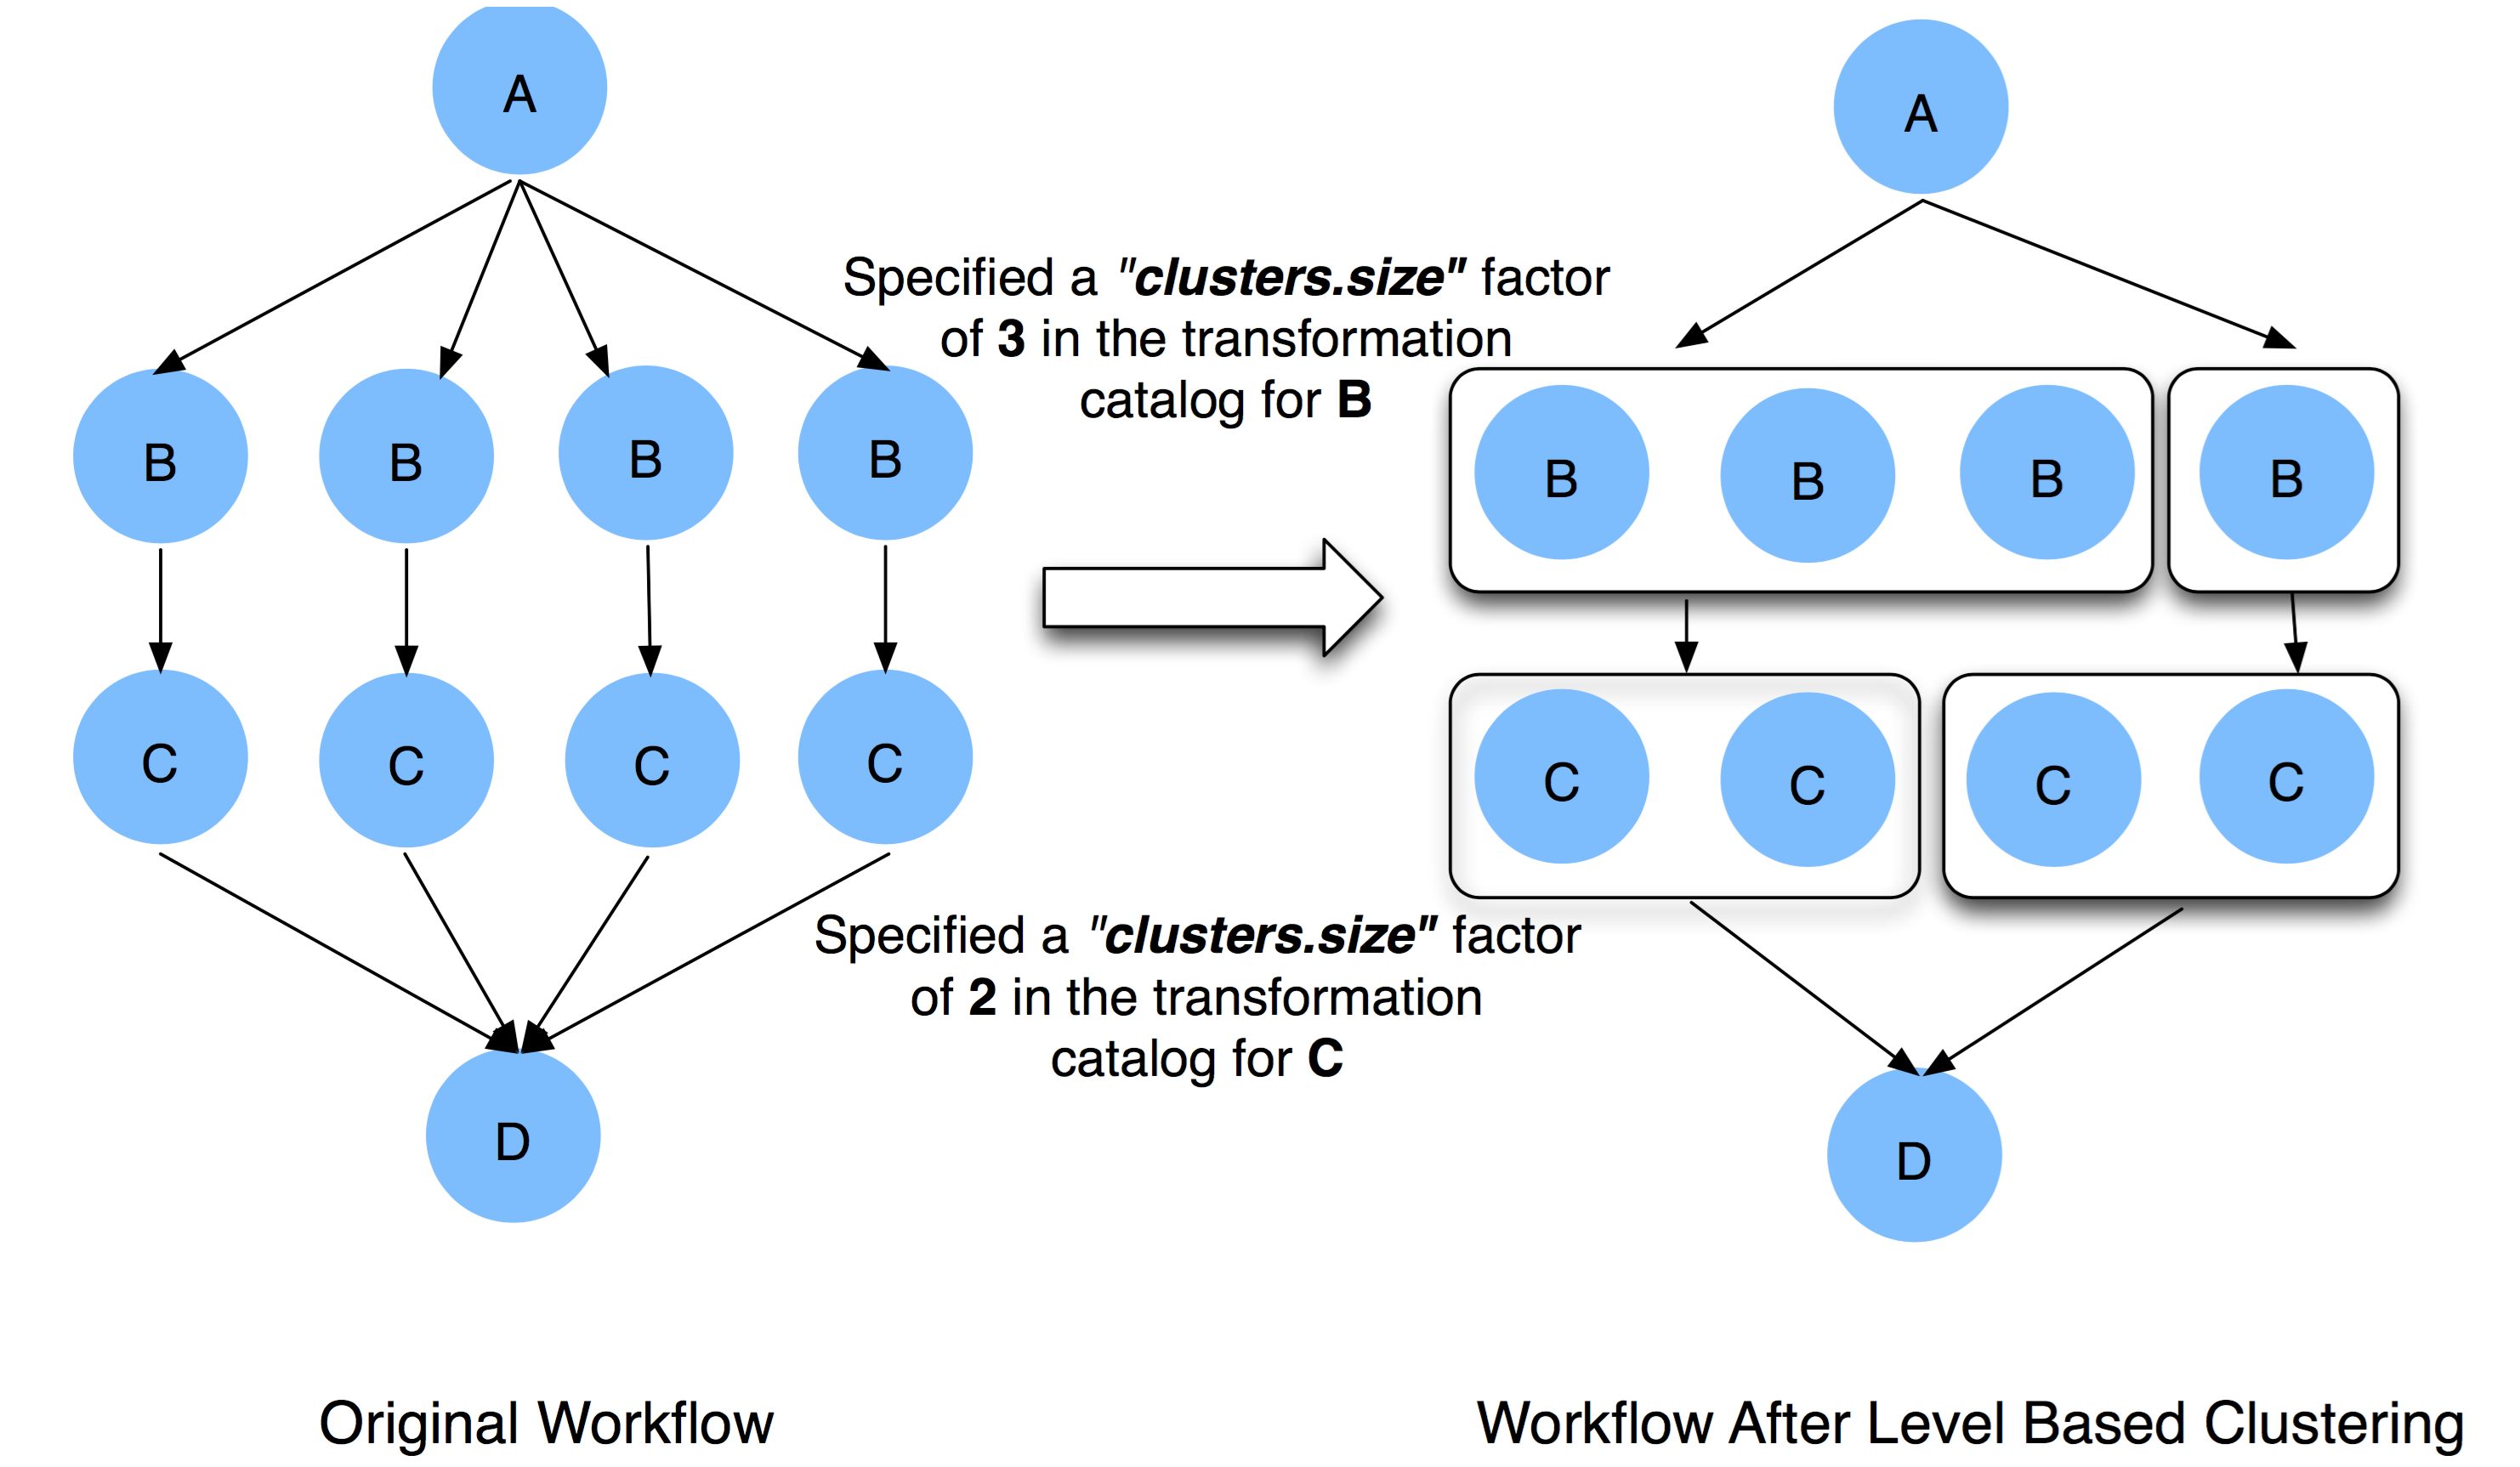
\includegraphics[scale=0.23]{HorizontalClustering.png}
	\caption{Level-based horizontal clustering targeting parallelisable tasks \cite{Deelman2013}.}
	\label{HorizontalClustering}
\end{figure}

\begin{figure}[h]
	\centering
		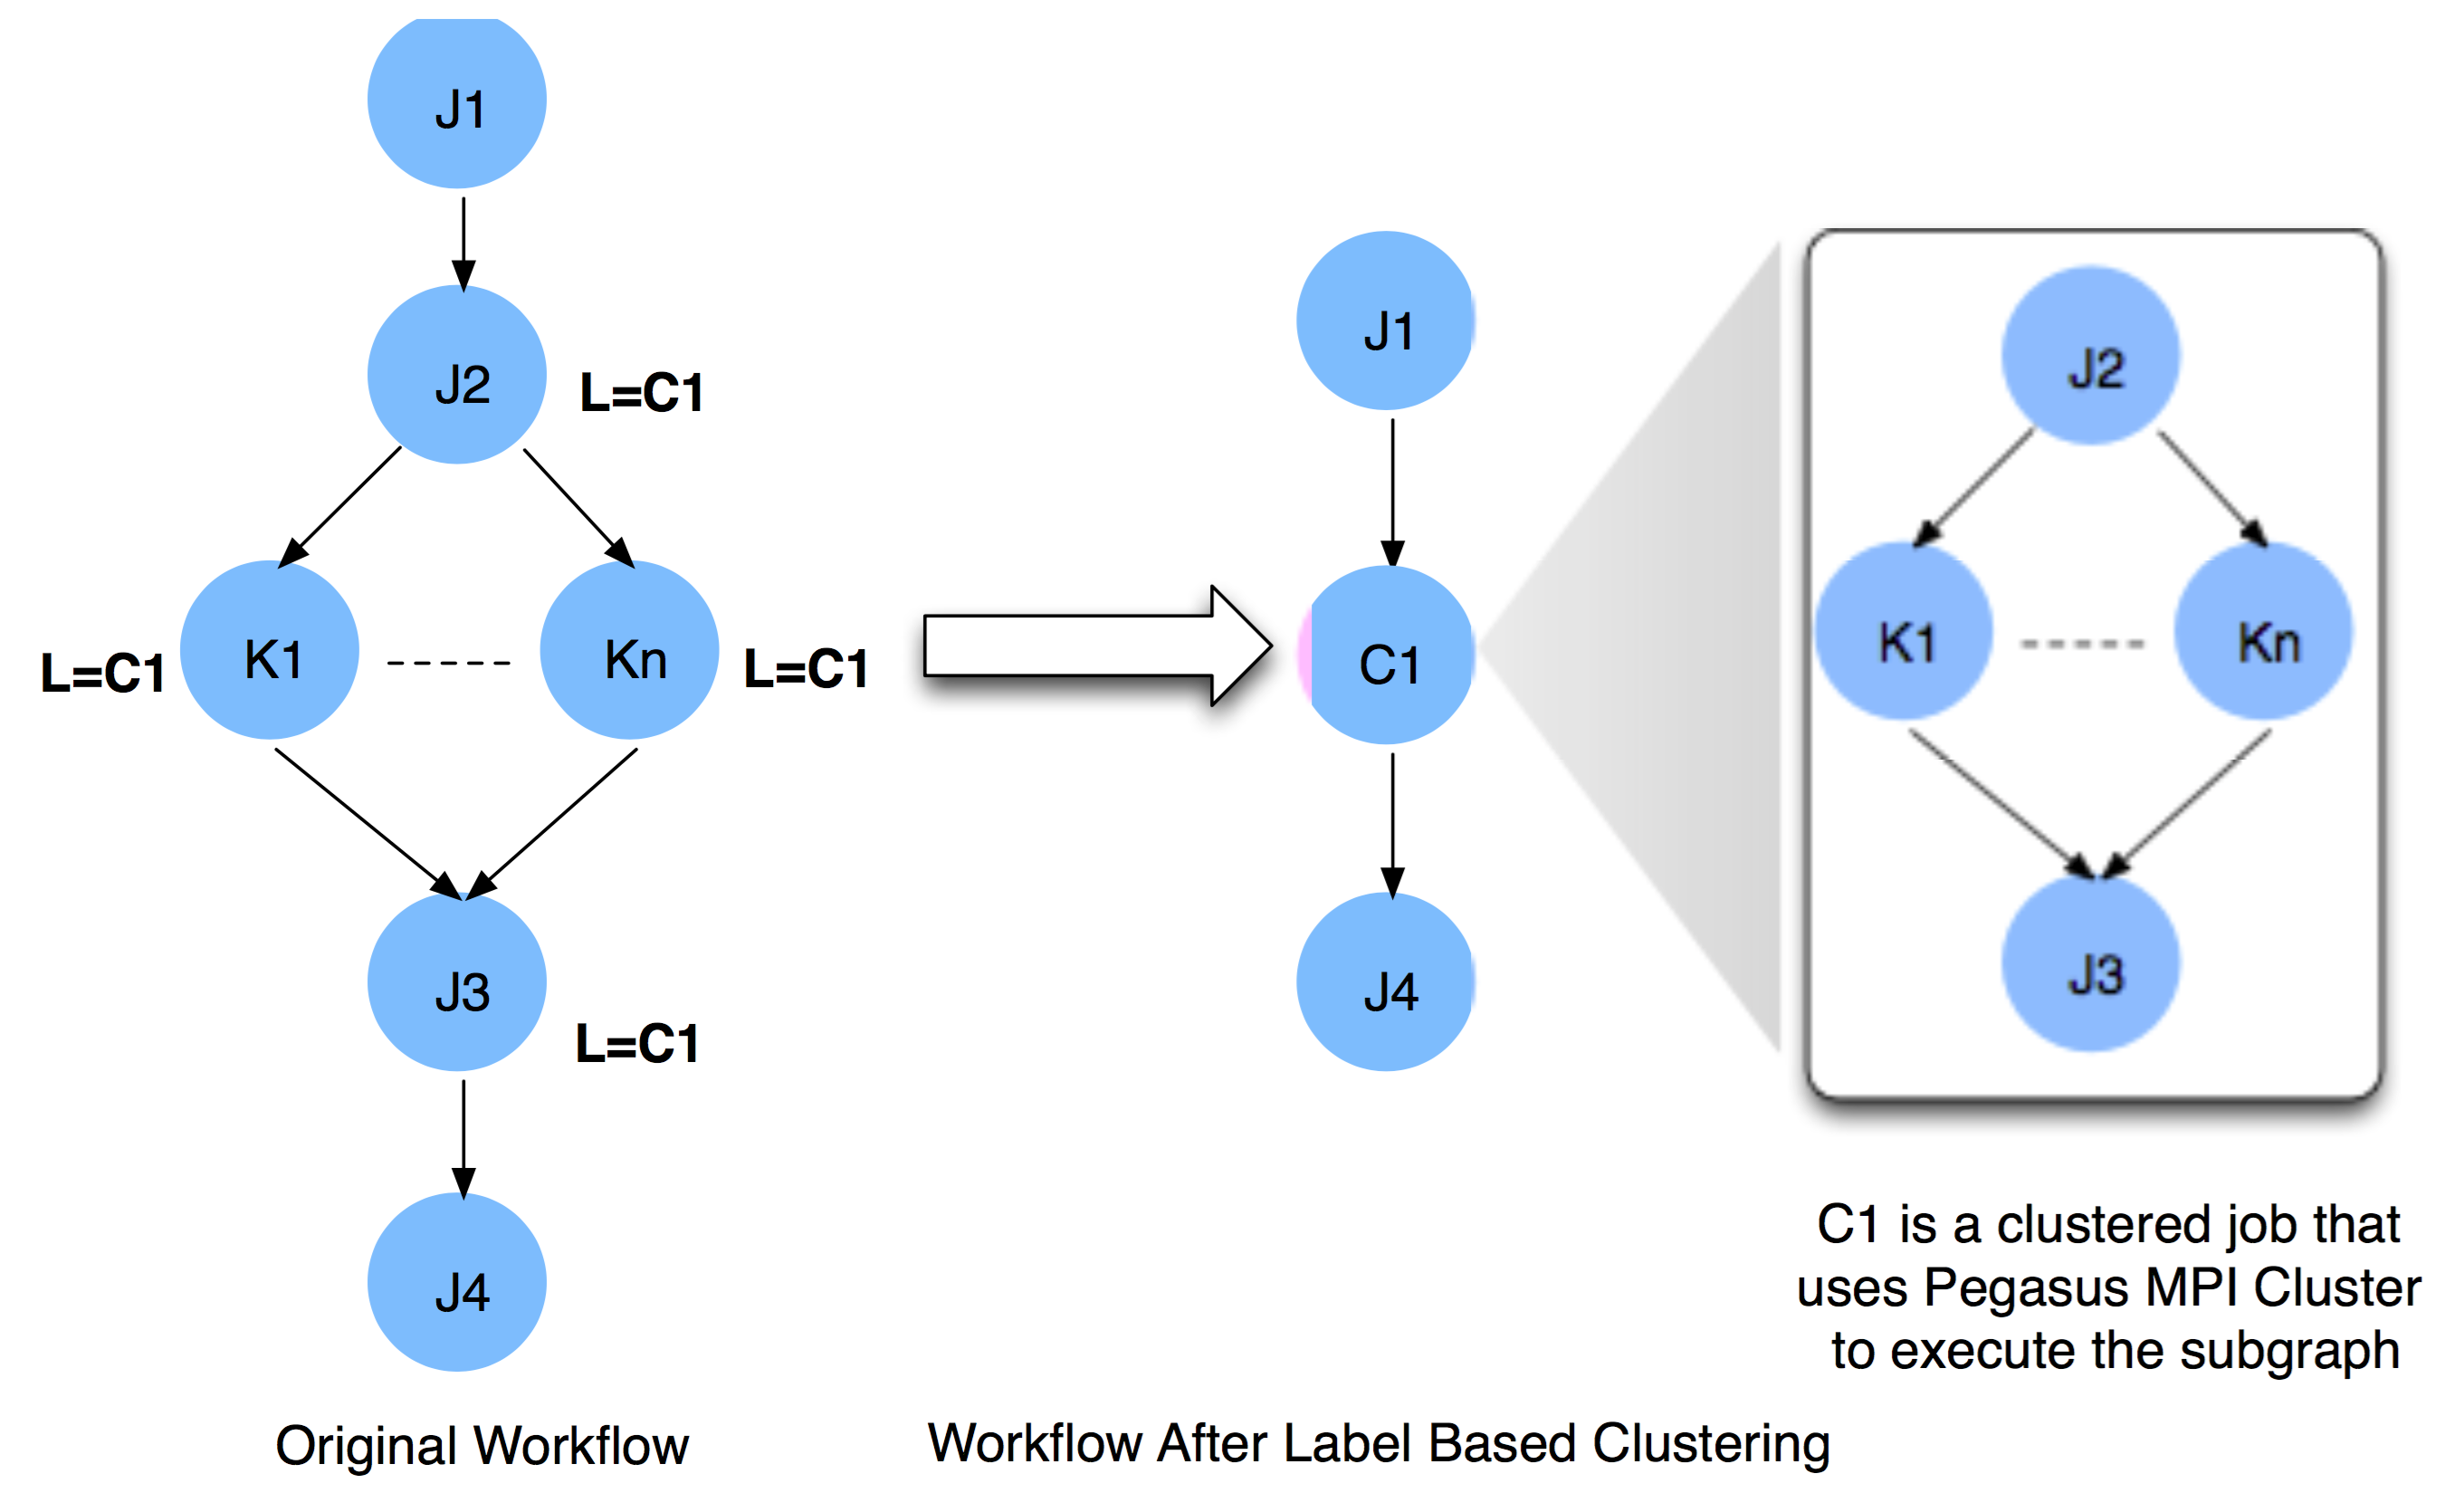
\includegraphics[scale=0.23]{LabelClustering.png}
	\caption{Label-based clustering \cite{Deelman2013}.}
	\label{LabelClustering}
\end{figure}

Although all the optimisations and design ideas discussed above apply to all distributed execution platforms, earlier deployments of Pegasus have confirmed several advantages of cloud environments. These include on-demand provisioning of resources and ability to easily ensure consistency of software installed on all the machines in a fleet \cite{Deelman2016}. 

However, further development of workflow management systems is needed in order to fully exploit cloud features such as automatic scaling of available resources. The main problem is that the load of instances occurs in the case of long-running jobs. Indeed, upscaling usually leaves unused extra resources, while downscaling is even more challenging because long individual tasks cannot be split up any further. Basic solutions involve only allowing automatic scaling on idle instances or when having many short-lived jobs, but this is definitely an area open to future work.

Despite the trend towards cloud-based systems, the process of running Pegasus workflows in the cloud has still not been fully automated. Users are required to manually configure the job submission host and worker nodes to run the required software \cite{PegasusTutorial}. At the moment, the technical barrier for harnessing the cloud from Pegasus is higher than grid-based options, that are usually specifically designed for running experiments and provide a preconfigured software stack.

\section{Cluster Deployment on Clouds}

In this section, we analyse some of the tools that can be used for creating a cluster from a set of instances provided in a cloud environment. The main motivation behind the investigation is that deploying a cluster running one of the environments already supported in OpenMOLE allows leveraging the existing infrastructure by simply delegating the work to a cluster running in the cloud. We believe that this is a sane approach for developing a functional prototype, which can later be improved by using native cloud APIs in case this is required due to slowdowns caused by the additional clustering layer.

Throughout the investigation, we focus on the features relevant to managing cloud infrastructures. We are interested in a tool that:
\begin{itemize}
	\item Supports most of the important cloud infrastructures (EC2, Google Cloud, OpenStack, CloudStack). We initially only target EC2, but we also intend to integrate with other platforms in the future.
	\item Is lightweight enough not to cause significant overhead on the performance of the instances in the cluster.
	\item Is open-source, since we plan to use it as part of GridScale. However, we also examine some commercial and proprietary systems to better educate our decision.
	\item Allows for effective automation in a concise manner by providing a clear and robust command line interface or API.
\end{itemize}

\subsection{StarCluster}

StarCluster \cite{StarCluster} is an open-source cluster management tool that has been successfully used in both open-source and commercial products. It comes as a command line tool that specifically targets cluster deployment on Amazon EC2 and provides flexible high-level configuration options.

By default, StarCluster provides a set of public AMIs that include a lightweight software stack for job scheduling, intra-cluster communication and common scientific data manipulation tasks. From a system administration perspective, the out-of-the-box StarCluster configuration includes:
\begin{itemize}
	\item NFS\footnote{Network FIle System} \cite{NFS} for sharing data between the instances in the cluster.
	\item The SGE job queuing and scheduling system.
	\item Security group setup for controlling the inbound and outbound traffic from the cluster.
	\item Password-less SSH between the nodes in the default security group.
	\item The possibility of attaching and mounting EBS drives to be used as NFS-shared storage by all the nodes in the cluster.
\end{itemize}

On top of this, the StarCluster AMI also contains tools like OpenMPI \cite{OpenMPI} and IPython \cite{IPython} for writing natively parallel applications. Other features revolve around various preconfigured software packages associated with high-performance computing development stacks, but they go beyond our use cases.

StarCluster relies heavily on the assumption that users prefer sensible defaults rather than extensive configuration. The standard installation requires a single \verb|start| command to set up a cluster with a given number of nodes on EC2 and new clusters are automatically configured with NFS and SGE support. Listed below are some of the most useful commands exposed by StarCluster:
\begin{itemize}
	\item \verb|start| launches a cluster as per the specification provided in the configuration file. It allows for many different variations of cluster creation, where instances can also be simply started but not provisioned with the default software. The user can also simply perform a dry run and simply simulate starting the cluster to prevent unexpected issues in production.
	\item \verb|terminate| completely purges the given cluster, shutting down all nodes and removing its previously created security group. If the cluster is backed up by EBS volumes, the root volumes of each node can also be deleted.
	\item \verb|sshmaster| and \verb|sshnode| allow for easy SSH access to all nodes in the cluster relying on the AWS keypair provided in the configuration file for authentication. Slave nodes are automatically numbered in a human-readable format - \verb|node001|, \verb|node002|, etc.
	\item \verb|put| and \verb|get| enable transferring files between the user's local machine and a running cluster, where they are instantly shared via NFS.
	\item \verb|createkey| is a useful for creating a new SSH keypair and simultaneously both saving it locally and importing it to the user's AWS account.
	\item \verb|addnode| and \verb|removenode| allow for manual upscaling or downscaling by launching new nodes and attaching them as slaves to the cluster or tearing them down.
	\item \verb|loadbalance| provides an automatic alternative for growing and shrinking the number of nodes in the cluster based on the load of jobs queued in SGE.
\end{itemize}

\textit{Elastic Load Balancing} is an important feature based on data extracted periodically from the monitoring component of SGE. Depending on the load of the queuing system, StarCluster automatically scales the size of the cluster by adding or removing instance nodes. This ensures that the number of idle jobs in the system is never excessively high, although it is unclear how the heuristic will perform when handling numerous short-lived or few long-lived tasks. 

The load balancing component allows choosing the minimum and maximum number of nodes that the size of the cluster can vary between, as well as its growth rate. The user can align this with domain knowledge about the job submission patterns, meaning that a cluster used to run a highly volatile number of short-lived jobs should adapt faster to the increase in requests and provision more instances at each monitoring iteration than a cluster used to run long-lived jobs. Other useful options include plotting the number of instances used by the cluster over time, the ability to allow the cluster a stabilisation time period during which the load balancer does not run, or automatically killing the cluster after a specific duration or when the job queue is empty.

StarCluster also provides a bidding strategy for provisioning EC2 \textit{spot instances} that allowed the StarCluster team to reduce instance renting costs by approximately 60\% over longer periods of usage. Spot instances allow users to rent currently unexploited resources from idle machines for a significantly lower price than the standard flat rate, with the drawback that access may be suddenly terminated when the original owner needs the computing power back. The framework deals with the caveat of losing access to the machine due to the current spot price becoming \textbf{higher?} than the maximum bid. However, the solution of simply rerunning the failed job on an on-demand instance might not be ideal in the context of long-running services or tasks.

Despite that tight coupling with specific components of the AWS ecosystem is undesirable, the close integration does bring quite a few advantages in terms of storage flexibility. StarCluster can use S3 and EBS interchangeably, with data from mounted EBS volumes being instantly accessible throughout the cluster.

\subsection{Elasticluster}

Elasticluster \cite{Elasticluster} is another open-source project aiming at simplifying managing clusters on cloud platforms. Although not as popular as StarCluster, it has similar goals and a focus on simplicity and is more generic by supporting all of Amazon EC2, Google Cloud and OpenStack. We do not intend to call from Scala the Python API that Elasticluster provides, so we will focus on the functionality provided by the command-line tool.

Given the more generic approach, Elasticluster makes fewer assumptions about the intentions of the user and requires more details to be set via the configuration file. It supports all of SGE, Slurm, Torque and PBS as scheduling systems. It uses Ganglia \cite{Ganglia} for monitoring and allows transparent configuration of its toolkit via Ansible \cite{Ansible}. Along with the division of nodes in a cluster in \textit{frontend nodes} and \textit{compute nodes}, the use of Ansible playbooks allows combining different setups for master and slave nodes. Modularity is achieved by creating the specification of the different blocks of the cluster independently (\textit{login}, \textit{cloud}, \textit{setup}, \textit{cluster}, \textit{storage}) and simply assembling them to deploy the instances.

Although not as feature-rich as StarCluster, Elasticluster offers the basic cluster management commands and some extra customisation options:
\begin{itemize}
	\item \verb|start| launches the cluster and automatically runs Ansible to configure it unless the user specifically requests not to.
	\item \verb|stop| kills the cluster without checking whether it is currently in use, which makes the tool require extra precautions on behalf of the user when managing the lifecycle of the client application.
	\item \verb|list-nodes| offers information about all nodes in a specific cluster.
	\item \verb|setup| allows the user to efficiently reconfigure the cluster from scratch without having to restart it and wait for instances to be recreated. It simply runs Ansible with respect to playbooks that have been added or updated by the user.
	\item \verb|ssh| and \verb|sftp| are used to obtain control of specific machines, upload and download files to and from the 
cluster.
	\item \verb|export| is used to save the local data about a cluster started from the current machine in a \verb|zip| file. A sensible but useful option is the ability to also store the local private and public SSH keys to the file.
	\item \verb|import| unzips and stores an exported cluster locally.
\end{itemize}

Although SGE is supported as in StarCluster, the main Ansible playbook we are interested is the one setting up Slurm, since it is the more popular, modern and actively maintained scheduling system. The Slurm playbook exports the \textit{/home} filesystem from the master node to all the slaves, ensuring shared storage. However, extra performance can be achieved by combining the Slurm playbook with the OrangeFS parallel virtual filesystem and mounting OrangeFS nodes as shared storage in the main cluster.


\todo[inline]{I changed all the SLURM to sentence case as it's the way they refer to it now}

A disadvantage of Elasticluster is that it does not support the native storage systems for its supported cloud platform providers, since Amazon and Google cloud instances usually report much better performance when coupled with storage on the same platform. Instead, Elasticluster has default support for GlusterFS \cite{GlusterFS}, Ceph \cite{Ceph} and the OrangeFS \cite{OrangeFS} filesystem. Although these options are performant, they suffer from not being as widely popular as the previously mentioned ones.

Elasticluster facilitates adding and removing nodes from the cluster, but does not provide the flexibility of StarCluster to dynamically control the load by provisioning instances on demand. This is a major disadvantage, since the responsibility for implementing the behaviour is transferred to the user, despite the fact that failure strategies would be more robust if incorporated within the tool itself.

\subsection{CfnCluster}

CfnCluster is a cluster management tool built by Amazon specifically to support running high performance computing  clusters using the entire stack of cloud services provided by AWS. This command line tool is free and open-source on its own, but it delegates most of the logic for administering the cluster to paid AWS services such as Amazon SNS\footnote{Simple Notification Service} \cite{SNS}, SQS\footnote{Simple Queue System} \cite{SQS}, CloudWatch \cite{CloudWatch} and Auto Scaling \cite{AutoScaling}.

The default installation is based on a provided AMI that ships with standard tools used for AWS administration. The configuration file allows extensive customisation and the possibility to enable various features needed for a job submission cluster:
\begin{itemize}
	\item A scheduler that can be any of SGE, Slurm, Torque and OpenLava\cite{OpenLava}.
	\item Shared filesystem by mounting and EBS volume on all nodes at a user specified location. Read-write access to resourced owned by the user in S3 is also enabled.
	\item Amazon Virtual Private Cloud (VPC) provisioning in order to operate a cluster whose networking layer is in complete control of the user and is in a logically isolated section of AWS.
	\item Security groups for a cluster-level firewall.
	\item Custom bootstrap actions that allow the user to run pre and post-startup configuration scripts on the master node.
\end{itemize}

Figure \ref{CfnNetworking} illustrates the sandboxing feature that isolates the master and compute nodes into subnets of the VPC.

\begin{figure}[h]
	\centering
		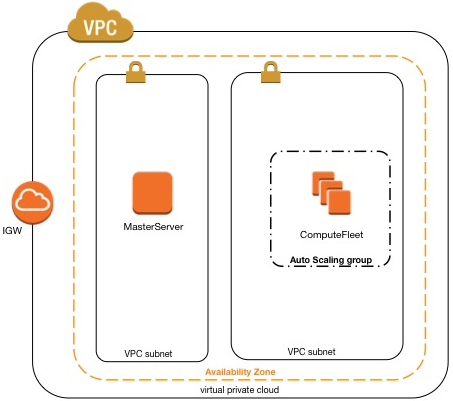
\includegraphics[scale=0.7]{CfnNetworking.png}
	\caption{Master and slave nodes isolated in two different Virtual Private Clouds \cite{CfnVPC}.}
	\label{CfnNetworking}
\end{figure}

Elasticity is achieved through the interplay of various Amazon cloud services. On cluster creation, a CloudWatch alarm monitoring the number of pending jobs is created. When the alarm is triggered due to many queued jobs, instances are added by the Amazon Auto Scaling service up to a maximum defined by the \verb|max_queue_size| config parameter. On the other hand, idle machines are identified using a \verb|nodewatcher| daemon that monitors load and signals the possibility to reduce the compute fleet size to a minimum of \verb|min_queue_size| instances. Figure \ref{CfnScaling} demonstrates the processes described above.

CfnCluster is a production-ready and reliable tool. However, it is completely one-dimensional since it focuses entirely on Amazon software and incurs extra costs by using many other AWS services, which could have otherwise been implemented as features of the tool itself. Although the costs of the individual cloud services supporting CfnCluster is not high, the overall cost is higher. An estimate for the added cost introduced by ClowdWatch alarms only is \$3.50 per month per instance, compared to the \$18.72 per month for renting a \verb|t2.small| instance \cite{AWSPricing}. This implies an added cost of 19\% that can by avoided by instead using StarCluster or Elasticluster.

\begin{figure}[h]
	\centering
		\subfloat[][Fleet size management.]{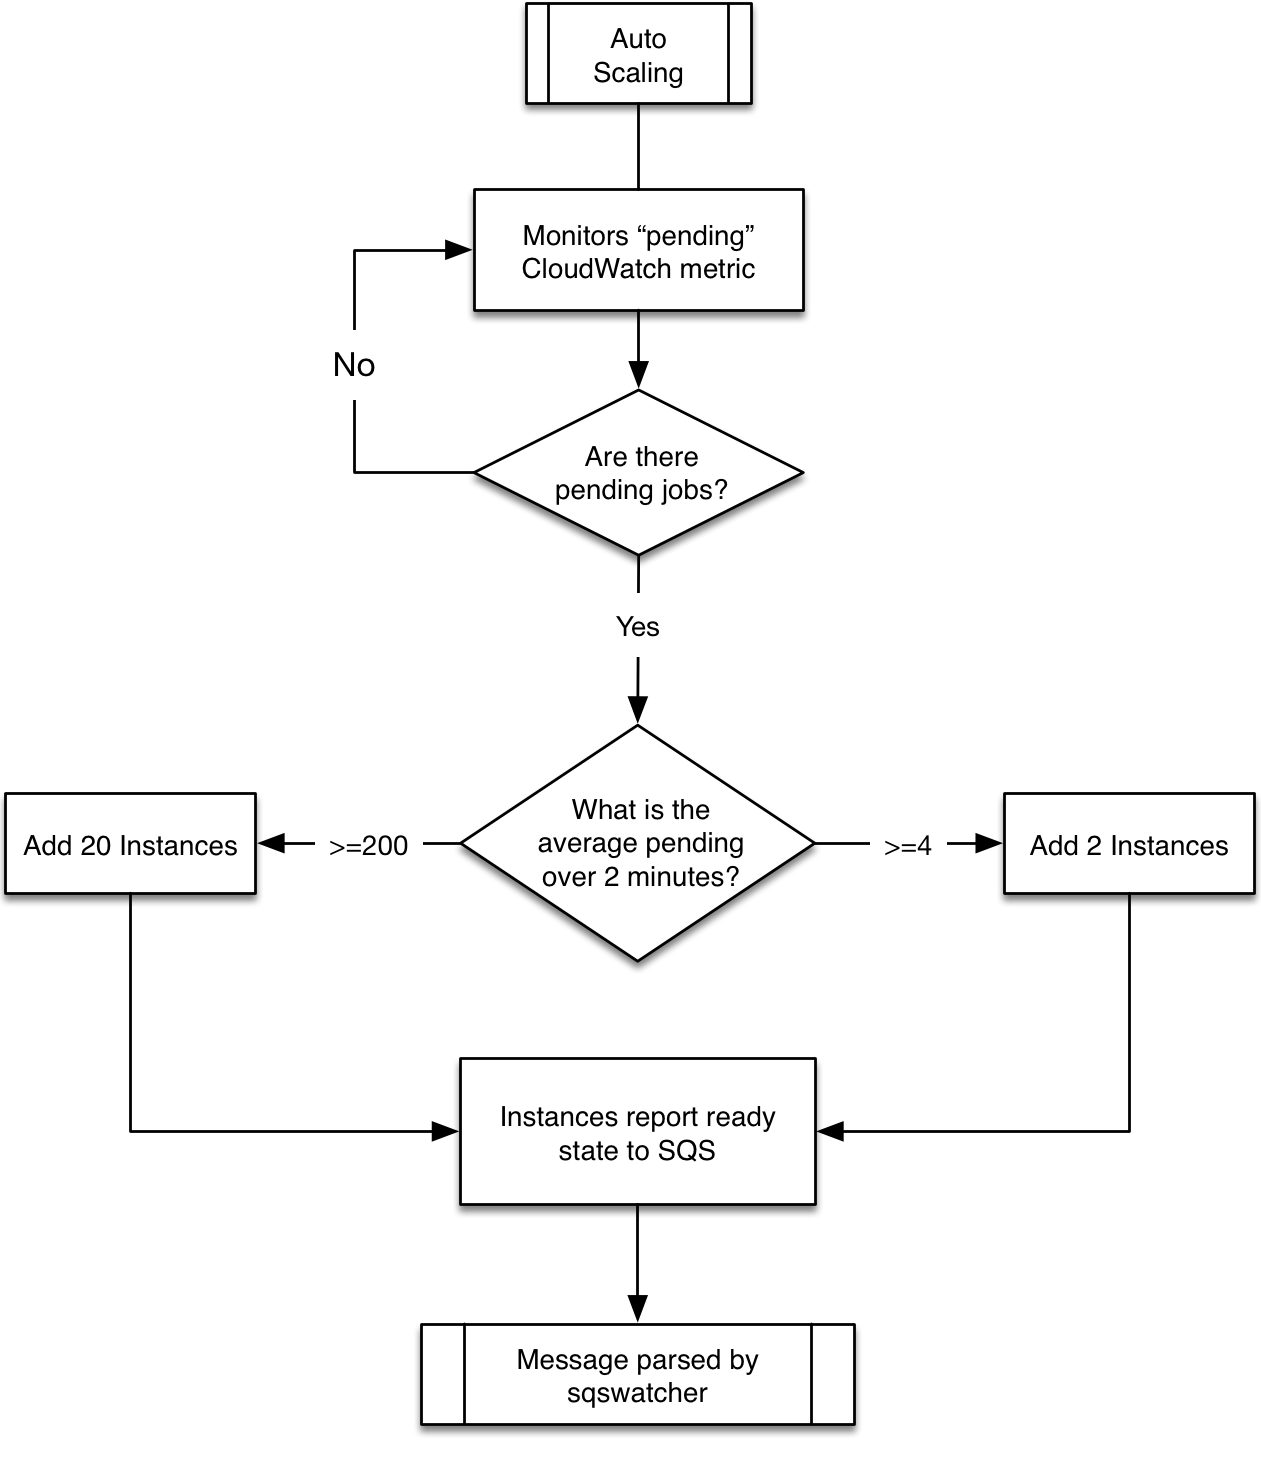
\includegraphics[width=0.7\linewidth]{CfnAutoScaling.png}}
		\subfloat[][Node activity daemon.]{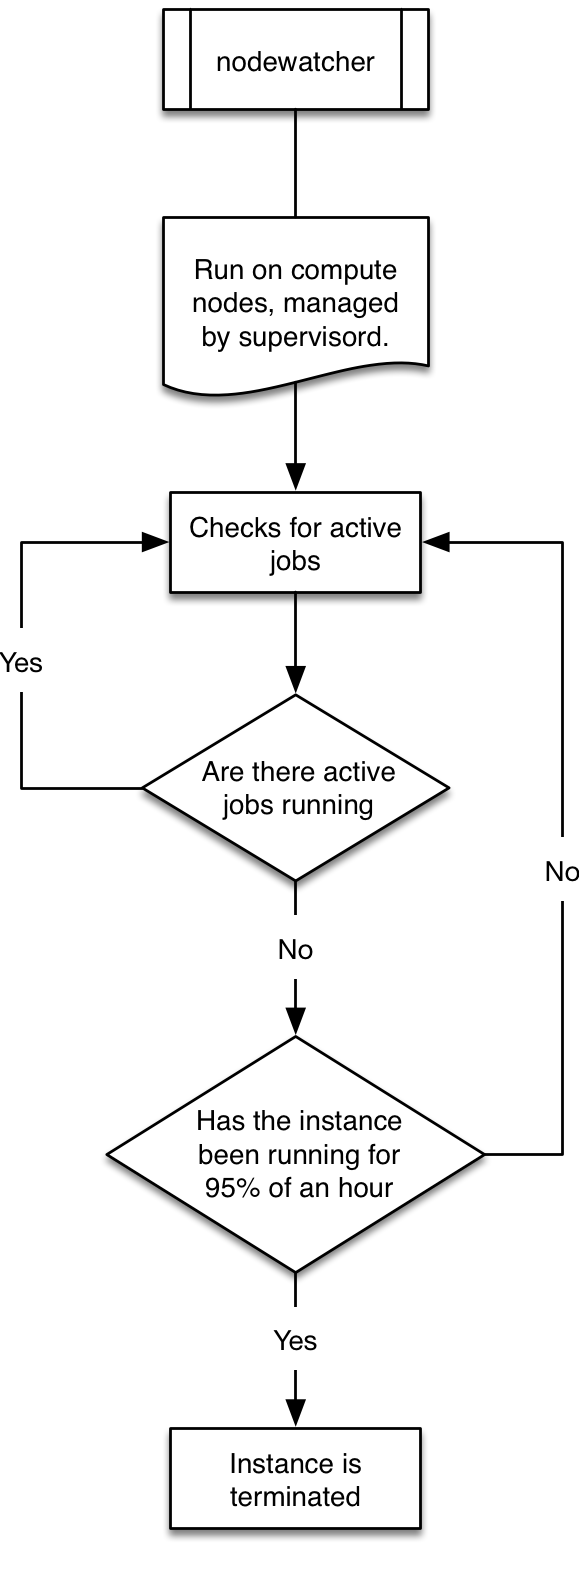
\includegraphics[width=0.3\linewidth]{CfnNodewatcher.png}}
	\caption{Auto Scaling monitoring diagrams \cite{CfnProcesses}.}
	\label{CfnScaling}
\end{figure}

\subsection{Apache Jclouds}

Apache Jclouds \cite{jclouds} is an open-source Java library that unifies the cloud services APIs for most mainstream commercial and open-source cloud providers, providing a starting point for an implementation that would be concerned with more fine-grained control of cloud specific features.

Although it requires more extensive configuration, it supports most commercial and open-source clouds (Amazon EC2, Google Cloud, Microsoft Azure, OpenStack, CloudStack), while not compromising highly provider-specific features. This is achieved by having highly flexible services for computation or advanced tasks like load balancing by using on-demand provisioning features of the clouds. For EC2, our main point of interest, Jclouds supports all type of storage provided by AWS, including EBS for low-latency services, S3 for low costs and Glacier for long-term storage.

Jclouds currently provides three main abstractions that facilitate writing code agnostic to particular cloud vendor APIs:
\begin{itemize}
	\item The \textit{ComputeService} layer unifies services providing computational power offered by different providers like Amazon EC2 or Google Compute Engine. The abstraction builds on top of the native APIs provided by the vendors and offers various features:
	\begin{itemize}
		\item The location aware API ensures that accessing resources placed in different geographic locations does not require maintaining multiple connections and managing multiple access objects. This permits a more clear organisation of code that oversees running virtual instances in multiple regions.
		\item Basic cluster management support is offered by allowing the creation of groups of nodes instead of individual machines. Each group benefits from an automatically bootstrapped firewall that can be configured to regulate the traffic to the group as desired. Running scripts on all the machines in a group is also simplified through the existence of execution primitives and sensible exception types used to handle remote errors.
		\item SSH key management for nodes launched using the API - specified SSH keys are copied to instances on startup.
		\item Focus on testability - the library provides a stub compute service that mimics the behaviour of a remote execution environment for each provider, simplifying the task of writing tests for the top-level application.
	\end{itemize}
	\item The \textit{BlobStore} abstraction provides a portable way of accessing key-value stores such as Amazon S3, Google Cloud Storage or Microsoft Azure Blob Storage. Features are also location-aware and focus on unifying methods of accessing different types of storage:
	\begin{itemize}
		\item The \textit{filesystem} provider can be used to write data to memory, local disk or cloud blob storage using the same API.
		\item The \textit{in-memory} provider allows testing without the need for real credentials by stubbing in the memory of the local machine for the remote storage.
	\end{itemize}
	\item The \textit{LoadBalancerService} abstraction is a beta feature that aims to distribute the workload among nodes created in groups.
\end{itemize}

Listing \ref{ComputeService} shows an example of using the \verb|ComputeService| abstraction. After the access object is built from the provider preference and credentials, launching the instance from the template configuring options such as the operating system, memory requirements or opening specific ports for external communication.

\begin{listing}[h]
	\centering
	\begin{minipage}{11.6cm}		
		\begin{minted}[frame=single,framesep=2mm,baselinestretch=1.15,fontsize=\small,linenos]{scala}
ComputeService compute = ContextBuilder.newBuilder("aws-ec2")
    .credentials("identity", "credential")
    .buildView(ComputeServiceContext.class)
    .getComputeService();

Template template = compute.templateBuilder()
    .osFamily(OsFamily.UBUNTU)
    .minRam(2048)
    .options(inboundPorts(22, 80))
    .build();

compute.createNodesInGroup("jclouds", 1, template);
		\end{minted}
	\end{minipage}
	\caption{Instantiating an Amazon EC2 instance using ComputeService \cite{jclouds}.}
	\label{ComputeService}
\end{listing}

Obtaining the access object for a \verb|BlobStore| is similar. Uploading data to the blob requires first creating a container and is straightforward after input data is parsed.

\begin{listing}[h]
	\centering
	\begin{minipage}{12.5cm}
		\begin{minted}[frame=single,framesep=2mm,baselinestretch=1.15,fontsize=\small,linenos]{scala}
blobStore = ContextBuilder.newBuilder("aws-s3")
             .credentials("identity", "credential")
             .buildView(BlobStoreContext.class)
             .getBlobStore();

blobStore.createContainerInLocation(null, "test-container");

ByteSource payload = ByteSource.wrap("test-data".getBytes(UTF_8));
blob = blobStore.blobBuilder("test")
    .payload(payload)
    .contentLength(payload.size())
    .build();

blobStore.putBlob("test-container", blob);
		\end{minted}
	\end{minipage}
	\caption{Uploading data to Amazon S3 using BlobStore \cite{jclouds}.}
	\label{BlobStore}
\end{listing}


Jclouds is a useful toolkit for managing computing and storage resources rented from different cloud providers without delving to deep into vendor libraries. However, it does not provide full cluster functionality, such as installing and configuring a job scheduling system or a shared filesystem. Implementing the whole cloud access layer using Jclouds would require duplicating a large part of the logic existing in tools already tested in production settings like Elasticluster, Starcluster or CfnCluster.

\subsection{Mesos}

Mesos \cite{Mesos} is an open-source cluster management system that provides abstractions of resources like processing power, memory or storage gathered from individual machines. Its aim is to offer a platform for creating safe, scalable and fault-tolerant distributed systems while programming against a simple API that allows treating an entire fleet of cloud instances as a shared supply of resources.

Mesos can be described as a kernel for distributed systems. Its architecture is similar to the one of the Linux kernel, but revolves around working with distributed resources. Applications that take advantage of the APIs exposed by Mesos are known as frameworks and common examples include platforms for batch job scheduling, processing big data, managing data storage or hosting long-running jobs such as web servers. Figure \ref{MesosArch} shows the how Mesos mediates the access of high-level frameworks to fragmented low-level resources.

\begin{figure}[h]
	\centering
		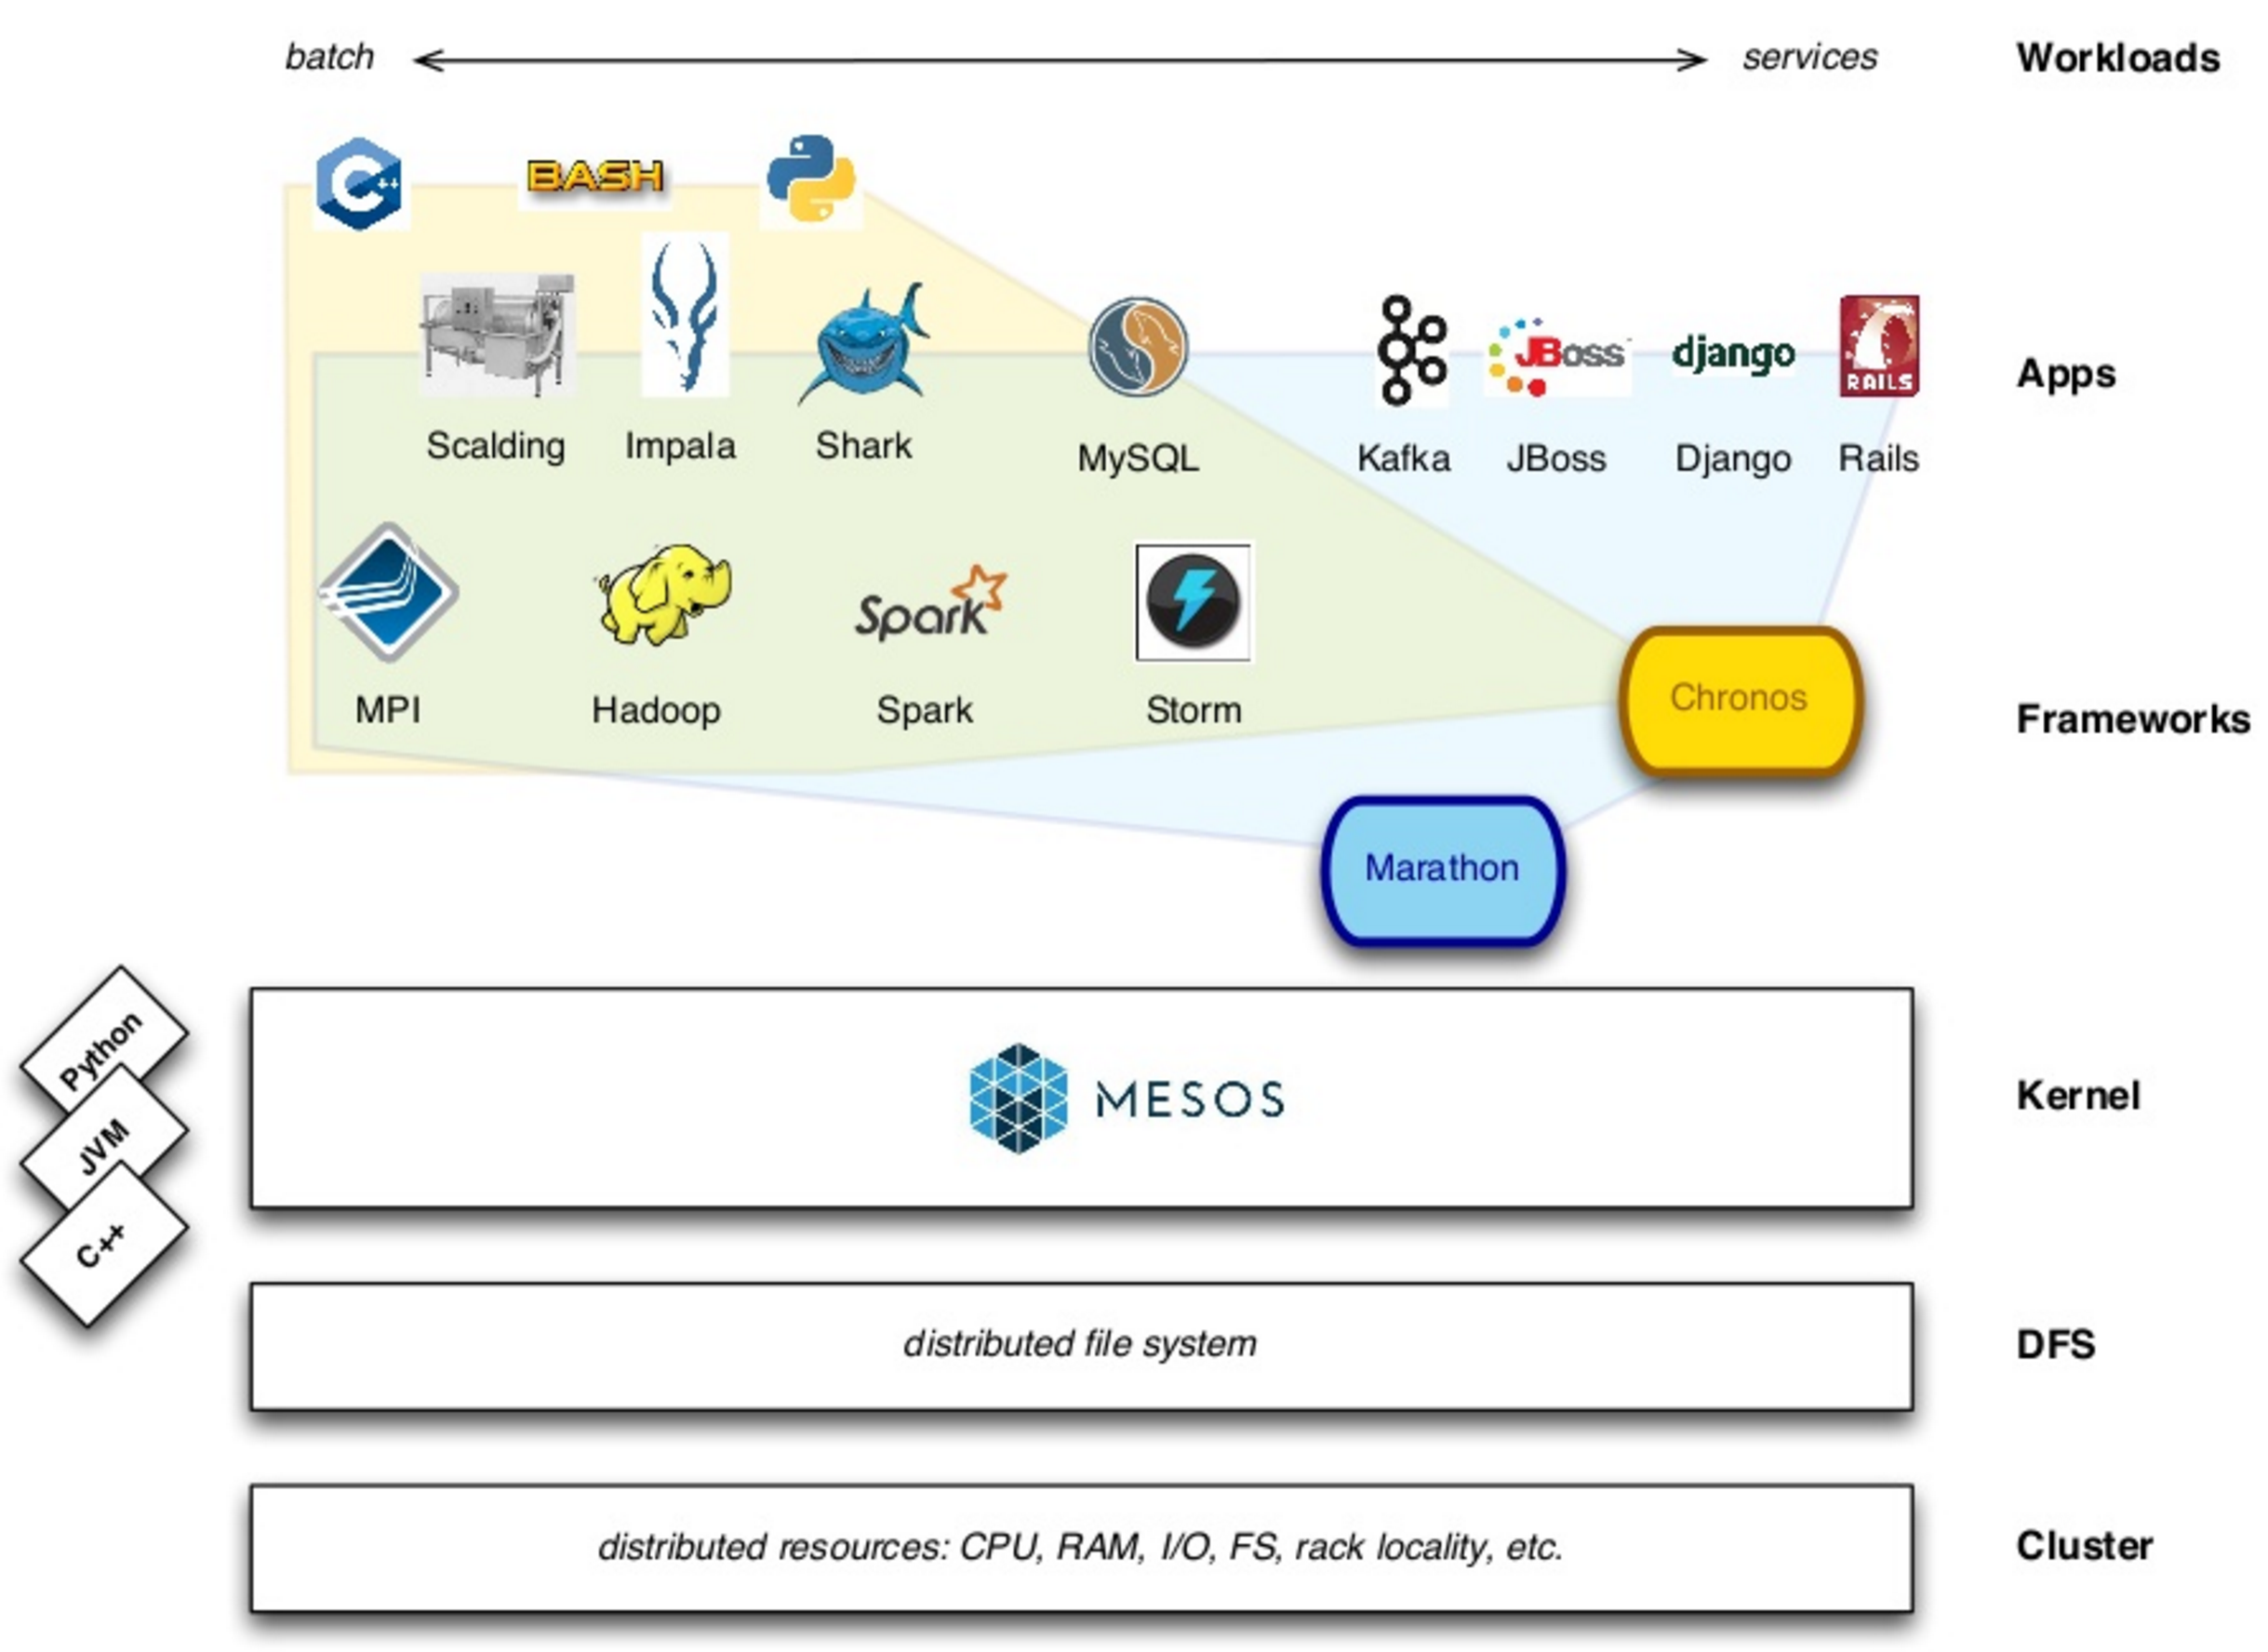
\includegraphics[width=1\linewidth]{MesosArch.png}
	\caption{Mesos architecture \cite{MesosArch}.}
	\label{MesosArch}
\end{figure}

The key advertising points for Mesos are its scalability tested in commercial applications to up to 10.000 nodes and its layered architecture that supersedes classic resource scheduling and distribution systems that maintain the whole state of the underlying infrastructure. Instead, Mesos completely handles resource unification and only requires blocks on top of it to deal with primitives such as resource offers and describing tasks that need to be executed on slave nodes in a cluster.

\subsubsection{Chronos}

Chronos \cite{Chronos} is a job scheduler that aims to be a modern redesign of the classic Unix utility Cron \cite{Cron}. Although Cron is mainly intended for performing single repetitive tasks and is typically used for scheduling system administration and maintenance tasks at regular time intervals, Chronos expands the feature space by also supporting job execution chains where jobs are triggered by finalisation of their dependencies. 

Chronos is built as a framework on top of Mesos and it benefits from the fault tolerance and scalability provided by the underlying distributed kernel and resources.

\begin{figure}[h]
	\centering
		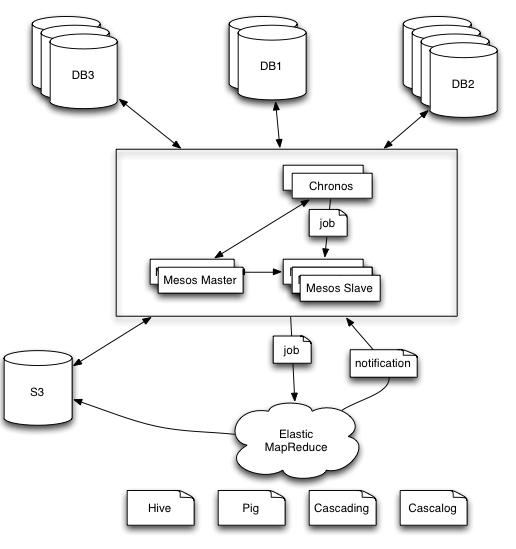
\includegraphics[width=0.9\linewidth]{ChronosArch.png}
	\caption{Chronos architecture \cite{ChronosArch}.}
	\label{ChronosArch}
\end{figure}

Figure \ref{ChronosArch} shows how Chronos fits in a system where it communicates with the Mesos master to allocate resources, which are then used to execute designated jobs. In the case when a Mesos cluster is deployed on AWS, the tasks leverage highly segregated compute power to perform big data processing using Elastic MapReduce \cite{EMR} and storage backed up by S3.

Chronos can aggregate statistics regarding the status of scheduled jobs batches, as well as details on individual executions. It also provides a web dashboard that can be used to manage jobs interactively, but our interest lies along the REST API for automation purposes. The simplest way to deploy and configure Chronos along with Mesos is by using Mesosphere DC/OS \footnote{Datacenter Operating System} \cite{DCOS}.

\subsubsection{Mesosphere DC/OS}

Mesosphere DC/OS is a distributed operating system using Mesos as its kernel and it facilitates the installation and orchestration of frameworks consuming the Mesos API. Figure shows the analogy between this setup and operating systems running on the Linux kernel.

\begin{figure}[h]
	\centering
		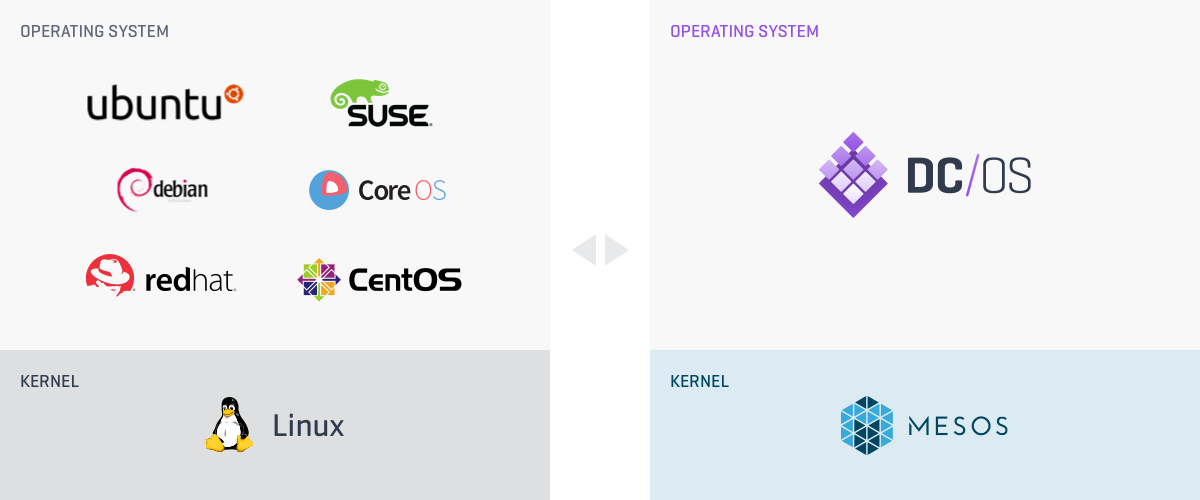
\includegraphics[width=0.9\linewidth]{DCOSArch.png}
	\caption{Mesosphere DC/OS architecture \cite{DCOS}.}
	\label{DCOSArch}
\end{figure}

DC/OS comes with out-of-the-box support for configuring clusters relying on instances provisioned from AWS and Microsoft Azure. By having DC/OS install Chronos, we can start executing jobs remotely using AWS resources. The community edition of the product is fully open-source and free to be used for non-enterprise purposes. However, for our use case this solution suffers from the same problem as CfnCluster, namely the extra cost induced by delegating all the elastic scaling work to services like Amazon Auto Scaling. 

Although DC/OS would not add extra costs directly, it does require more powerful bootstrap, master and agent nodes than either of Elasticluster, Starcluster or CfnCluster. Table \ref{DCOSPricing} shows the hourly price of operating an Amazon EC2 cluster with the minimum required specifications. In comparison, the cost of a \verb|t2.small|| instance that can be used as both a master and compute node in a Starcluster or Elasticluster installation with EBS volumes mounted for shared storage is \$0.026 per hour. This leads to a 10x cost increase only for operating a single master node and ignoring the fact that DC/OS in fact recommends running 3 simultaneous master nodes for optimal performance\footnote{All prices are quoted as per May 2016}.

\begin{table}[h]
\centering
\begin{tabular}{ccc}
\textbf{Node role} & \textbf{Required instance} & \textbf{Price (\$ per hour)} \\ \hline
\multicolumn{1}{|c|}{Bootstrap} & \multicolumn{1}{c|}{m3.2xlarge} & \multicolumn{1}{c|}{0.532} \\ \hline
\multicolumn{1}{|c|}{Master} & \multicolumn{1}{c|}{m3.xlarge} & \multicolumn{1}{c|}{0.266} \\ \hline
\multicolumn{1}{|c|}{Agent} & \multicolumn{1}{c|}{r3.large} & \multicolumn{1}{c|}{0.166} \\ \hline
 & \multicolumn{1}{c|}{} & \multicolumn{1}{c|}{0.964} \\ \cline{3-3} 
 &  & Total
\end{tabular}
\caption{Prices of EC2 nodes with DC/OS minimum performance requirements \cite{DCOSReq, AWSPricing}.}
\label{DCOSPricing}
\end{table}

In conclusion DC/OS is a highly reliable tool for operating clusters in the cloud, but from cost-effectiveness perspective its features only shine when used at massive scale. In our use case, where jobs are more numerous rather than particularly CPU-intensive, Starcluster and Elasticluster are better candidates and can produce similar results for a lower investment.